\todo{I would put more references into this Chpater.}
In Chapter~\ref{ch:pes-statistics}, we saw that the photoemission statistics are influenced by the characteristics of the light source, that exhibit well-defined statistical properties. Understanding these specific characteristics can be helpful in designing tailored, model-based denoisers. For Poisson noise, we employed the Anscombe transform combined with \gls{BM3D} (\cref{sec:poisson-noise-model}). While the Anscombe transform is capable of stabilizing Poisson-distributed noise into approximately Gaussian noise for moderate to high counts, it is less effective for very low counts ($<3$), where the approximation breaks down. Similarly, a \gls{VST} tailored for \gls{NB} statistics in conjunction with \gls{BM3D} could be more effective to reduce noise.

Model-based approaches such as these can be powerful but assume that the noise characteristics are accurately known and that the underlying signal conforms to the priors encoded. However, \gls{FEL}-based photoemission experiments involve complex and heterogeneous noise sources. Factors such as long-term fluctuations in \gls{FEL} intensity (\cref{section:fel-stats}), advanced detector designs (\cref{section:8s-dld}) and environmental variations can lead to deviations from idealized models like Poisson or \gls{NB} noise prior. Adapting model-based methods to account for these complexities requires significant effort and may still fall short when dealing with unknown or dynamically changing noise patterns.

Unlike model-based methods, which depend on predefined assumptions about the noise and other image priors, machine and deep learning methods \todo{``machine and deep learning methods'' sounds like machine learning and deep learning are different things, but the latter is just a special case of the former} can learn these relationships directly from data. This data-driven approach allows deep \todo{Now there is no mention of machine learning anymore. Perhaps the easiest would be to simply drop the term machine learning above and only talk about deep learning.} learning models to handle diverse and complex noise distributions, including those that are non-standard, multi-modal, or vary across a dataset. Furthermore, \gls{CNN}-based architectures excel at extracting non-linear and hierarchical features from such \todo{It's not clear what this ``such'' is referring to here. In this paragraph you didn't specify data sets. I assume you mean data drawn from complex noise distributions, but you don't explicitly say that.} high-dimensional data, structures typical of \gls{MPES} datasets. This allows to take advantage of the spatial and temporal correlations across multiple dimensions more effectively than many traditional approaches.

Machine learning can be broadly categorized in two categories: the \textit{supervised} and the \textit{unsupervised} setting. In supervised learning, the experience (\textit{model}) is learned by exposure to data containing information additional (labeled data) to what the model is supposed to map\todo{This is a somewhat implicit, somewhat complicated way to describe this. I think it would be easier if you first state the task, i.e., to learn a mapping, and you do that based on given input/output pairs, i.e. the training data.}. The exposure to such data, called \textit{training}, enables the model to establish a relationship between the inputs and their corresponding outputs. The model’s expertise can then be used to map new inputs to their corresponding outputs. In the context of image restoration, the model can gain expertise from pairs of corrupted and clean images, and then use this expertise to restore other corrupted images.

Conversely, in the unsupervised setting, the model is exposed to the data without any labeled information, and the model is supposed to learn the underlying structure of the data. In context of image restoration, that would imply only giving the model the corrupted images, and expecting to map to the desired target--the clean image\todo{Do you have specific unsupervised deep learning approaches for image restoration in mind? It's quite hard to imagine how this is supposed to be done in an unsupervised manner from this description.}.

This chapter, we will discuss the foundations of \todo{insert ``machine'' of ``deep'' here (depending on how you resolve the comments above)} learning, covering the elements of how and why learning works. This is general to both the supervised and unsupervised setting. There the concepts of \textit{hypothesis class}, \textit{capacity}, \textit{realizability}, and the concept of \textit{generalization} capability are discussed. Then we take a look at a statistical learning\footnote{Machine learning and statistical learning are many times used interchangeably but the latter places more emphasis on the statistical properties of the learning algorithms, and the former on the algorithmic aspects.} paradigm known as \textit{\gls{ERM}}, aiming to minimize the training error/empirical risk. \Gls{ERM} comes with its own set of challenges, such as overfitting in hypothesis spaces with high \textit{capacity}, which can be mitigated by \textit{regularization}. 

We discuss the combination of \textit{\gls{CNN}} and \textit{Autoencoders}, commonly used in image restoration tasks. Later, \gls{noise2noise}, a learning framework for image restoration not requiring clean images, introduced by \citeauthor{lehtinenNoise2NoiseLearningImage2018}, is discussed. To fully explain this framework, we look at the \textit{loss function} that allows this paradigm to work. We apply this training scheme using the concrete realization \texttt{UNET3D} architecture\todo{the grammar here sounds slightly off}, the 2D variant introduced first by \citeauthor{ronnebergerUNetConvolutionalNetworks}.

These methods are then applied to train a model that maps incomplete \todo{incomplete in which sense? Aren't you just using short exposure time data as input? Is this what you mean with incomplete? To me, incomplete would mean something different from short exposure / high noise. Or is this refferring to the fact that many pixels have no electron counts because of the short exposure? This should be made clear.} observations from \gls{PES} to the true multidimensional image, with $d=3$ dimensions. The aspects of data generation, training, and evaluation are henceforth, discussed in detail.

Much of the foundational concepts discussed are based on \cite{shalev-shwartzUnderstandingMachineLearning2014a,jamesIntroductionStatisticalLearning2013,tibshiraniElementsStatisticalLearning,goodfellowDeepLearning2016}.

\section{Foundations of Learning}
Statistical regression is a classical example of a learning algorithm, where the goal of regression is to learn a function that maps the input data to the output data.
Let us approach the image restoration problem from this perspective. Using the general observation model defined in \cref{eq:observation-model}, the learning problem is then to find a hypothesis $h$ \todo{Explaining why this is called hypothesis could be helpful.} hat maps the degraded image $X$ to the true image $Y$ that generalizes well.
\begin{equation}
    h: X \mapsto Y
\end{equation}

In machine learning, we \todo{This is a context, where ``we'' sounds a bit off. It sounds like we don't do this in machine learning, but other might. I would phrase this in passive, e.g., ``no explicit assumptions are made''} do not make any explicit assumption of the \textit{data generating distribution} except that all instances of the data are \textit{\gls{iid}} and generated according to a distribution $\mathcal{D}$ i.e.\ $Y, X \sim \mathcal{D}$. Continuing forward, since the discussion is not restricted to images, we denote input and target as $x$ and $y$ respectively. 

\subsection{Generalization}\label{sec:generalization}
\Gls{generalization} refers to the ability of a learning algorithm to perform well on new, unseen data. The goal of learning is to find a hypothesis $h$ that generalizes well to new data\todo{Here one has to know that $h$ was chosen based on the training data.}. 

If the data generating distribution $\mathcal{D}$ is \gls{iid} and known\todo{But this is pretty much never the case, is it?}, the \textit{generalization error}/\textit{population risk} $\mathcal{R}(\theta)$, with model parameters $\theta$\todo{Before you can use the model parameters, you first need to mention that $h$ is parametrized with these parameters.}, can be minimized to find the optimal hypothesis $\hat{h}^*$. $\mathcal{R}(\theta)$ is defined as expectation taken across the data generating distribution $\mathcal{D}$, with the predicted output of a hypothesis $h(x; \theta)$ and the true output $y$:
\begin{equation}\label{eq:risk}
    \mathcal{R}(\theta) = \mathbb{E}_{(x, y) \sim \mathcal{D}} \left[ \ell(h(x; \theta), y) \right]
\end{equation}
\todo{$\mathcal{R}$ is not a good symbol for this, since you'll use $R$ for the regularizer below (which is a fitting symbol there). So $\mathcal{R}$ and $R$ look very related, but are very different.}
where the loss $\ell$ measures the difference between two quantities, such as of $h(x; \theta)$ and $y$.

Through optimization, the optimal hypothesis $\hat{h}^*$ \todo{Even if you know the distribution (which you don't), you would usually not find a global optimizer with numerical optimization. But you can desribe the optimal hypothesis as solution to an optimization problem.} can be found that minimizes the expected risk $\mathcal{R}$:\todo{It's also very unlikely that there is only one global optimizer, which is implied by $\hat{h}^* = \argmin$... To avoid this, you can write, $\hat{h}^* \in \argmin$...}
\begin{equation}\label{eq:risk-min}
    \hat{h}^* = \argmin_{h \in \mathcal{H}} \mathcal{R}(\mathcal{D}; \theta)
\end{equation}

\subsection{Hypothesis Class, Capacity and Realizability}
The hypothesis $h$ is chosen from a hypothesis space $\mathcal{H}$, where the hypothesis space $\mathcal{H}$ is the set of functions that the learning algorithm can choose from to approximate the true function. 
For example, in linear regression, the hypothesis space $\mathcal{H}$ consists of all possible \todo{Due to the ``$++ w_0$'', theare are not truely linear, but affine or affine linear.} linear functions\todo{From $\mathbb{R}^d$ to $\mathbb{R}$.}\footnote{We also already an example of a problem where the hypothesis space $\mathcal{H}$ is constrained to linear functions: the linear minimum \gls{MSE} estimator, Wiener filter discussed in \cref{sec:wiener-filter}.} of the form:
\begin{equation}\label{eq:linear-hypothesis}
   \mathcal{H} =  \left\{ h_{\mathbf{w}}(\mathbf{x}) = \mathbf{w}^\top \mathbf{x} + w_0 \mid \mathbf{w} \in \mathbb{R}^d, w_0 \in \mathbb{R} \right\}
\end{equation}
where $\mathbf{w}$ is the weight vector, $\mathbf{x}$ is the input vector, and $w_0$ is the bias term\todo{Saying ``the weight vector'' and ``the bias term'' implies that the reader already knows what this are. Here, you rather introduce names for $\mathbf{w}$ and $w_0$.}. 

The \textit{capacity} (the measure of size\footnote{The VC dimension and Rademacher complexity are two popular measures of capacity.}) of this hypothesis space is smaller than other \todo{This formulation would imply that all other hypothesis spaces have a larger capacity. I don't think this is what you mean.} hypothesis spaces such as polynomial class of functions. Choosing a hypothesis class with a larger capacity allows for more complex functions to be learned, but we will see that this comes with a trade-off.

We want to find a space that makes our learning problem \textit{realizable}. This means that there exists a mapping \todo{I would rather say ``element'' instead of ``mapping'' here.} in the hypothesis space that can perfectly model the true mapping. An example for an unrealizable problem is if the data generation function is a $\sin(x)$ function, but the learning algorithm has a linear hypothesis space\todo{I think you mean if the linear mappings are used as hypothesis space. The multiples of $\sin$ are a linear space (containing non-linear functions), where you example is realizable.}. In most real-world scenarios, the true space for complex data such as images is seldom known, and we forego the realizability condition\todo{I'm not sure if you need to discuss realizability if you don't use it anyway.}. This is the \textit{agnostic} learning setting. For classes with high capacity, even if they can not perfectly model the true function, they might approximate it well.

\subsection{Empirical Risk Minimization}\label{sec:erm}
When the true data distribution $\mathcal{D}$ is unknown, the population risk can no longer directly be minimized. Instead, we approximate it by minimizing the empirical risk\todo{It would be helpful if it already became clear in this sentence that the empirical risk is going to be defined in the following and nothing that the reader should already know.}. For a training set $\mathcal{S} = \left\{ (x_1, y_1), \ldots, (x_n, y_n) \right\}$ where $\mathcal{S} \sim \mathcal{D}^n$, and model parameters $\theta$, the empirical risk $\mathcal{L}(\theta; \mathcal{S})$ (also known as \gls{training_error}) is defined as:
\begin{equation}
    \mathcal{L}(\theta; \mathcal{S}) = \frac{1}{\lvert \mathcal{S} \rvert} \sum_{(x, y) \in \mathcal{S}} \ell(h(x; \theta), y),
\end{equation}
where $\ell$ is the loss function that measures the error between the predicted output $h(x; \theta)$ and the true output $y$\todo{You already defined $\ell$ and $h(x; \theta)$ before.}. \Glsxtrfull{ERM} finds the hypothesis $\hat{h}$ from hypothesis space $\mathcal{H}$ that minimizes the training error $\mathcal{L}$\todo{As above, there may be more than one global minimizer and numerical optimization will most likely only find a local one.}
\begin{equation}\label{eq:erm}
    \hat{h} = \argmin_{h \in \mathcal{H}} \mathcal{L}(\mathcal{S};\theta)
\end{equation}
by optimizing the model parameters $\theta$.
We shall later see that the assumption of having access to a true $y$ can be relaxed in the \textit{Noise2Noise} framework using $L_2$ (\gls{MSE}) as the loss $\ell$.

The gap between the $\mathcal{L}(\theta; \mathcal{S})$ and $\mathcal{R}(\theta)$ is known as generalization error and a hypothesis with a large gap generally implies \textit{overfitting}.

\subsection{Regularization}
The \gls{ERM} algorithm runs \todo{``has'' instead of ``runs''?} the risk of overfitting. This means that the hypothesis $\hat{h}$ might perform well on the training data $\mathcal{S}$ but poorly on new data drawn from the same distribution $\mathcal{D}$. Usually, this happens for rich hypothesis classes (high capacity)\todo{This ``rich'' / ``high'' is not absolute, but always relative to the size of the training data.}, or when $\mathcal{S}$ is not representative of $\mathcal{D}$ \todo{When can this happen? Not enough training data would be an obvious cause. Are there others you can think of? If not, you could just state ``not enough training data''.} and the \gls{ERM} algorithm chooses a hypothesis that is too complex\todo{What is the complexity of a single element of the hypothesis class supposed to be? I don't really have an idea what you could mean here. In your setting the hypothesis class will be networks of the same architecture with different weights. So you would say that depening on the weight values a given network is more or less complex?}. 

To counter this, \textit{regularization} techniques are used. A penalty term based on model parameters is added to prevent overfitting. The \gls{ERM} then finds the hypothesis $\hat{h}$ that minimizes the regularized loss function\footnote{This is also known as Regularizated Loss Minimization.}:
\begin{equation}
    \hat{h} = \argmin_{h \in \mathcal{H}} \left(\mathcal{L}(\theta; \mathcal{S})  + \lambda R(\theta) \right).
\end{equation}
where $R(\theta)$ is the regularization term that penalizes complex \todo{This would even imply that larger weight mean more complex, e.g., replacing $\theta$ by $2\theta$ increases the value of the regularizer, but I don't see how you could argue that $h(\cdot;2\theta)$ is more complex than $h(\cdot;\theta)$.} models, and $\lambda$ is the parameter controlling the trade-off between the training error and the regularization term. Common regularization techniques include $L_1$ (Lasso) and $L_2$ (Ridge) regularization\todo{If you throw out the names ``Lasso'' and ``Ridge'', you should hint where they come from. The meaning of $1$ and $2$ are obvious and need to explanation.}. $L_1$ regularization can be written as:
\begin{equation*}
    R(\theta) = \|\theta\|_1 = \sum{j} |\theta_j|
\end{equation*}
and $L_2$ regularization as:
\begin{equation*}
    R(\theta) = \|\theta\|^2_2 = \sum_{j} \theta_j^2
\end{equation*}
\todo{I think you have not once mentioned so far in this chapter that $\theta$ is a vector. You need this here in order to spell our these regularizers.}

Regularization can also be seen as a way of restricting the hypothesis space $\mathcal{H}$ by encoding prior knowledge into the model\todo{Which prior knowledge do the two example regularizers above encode?}. In the case of image restoration, it might be known a priori that the image is smooth, and  can encode this prior knowledge by adding a penalty term that penalizes sharp changes in the image\todo{Do you have an example reference where this is done?}.


\subsection{Uniform Convergence}
It is always possible that with a small probability, the training data is not representative of the data distribution $\mathcal{D}$. Hence, every learning algorithm has a confidence and accuracy level that\todo{What are the confidence and accuracy levels? If you talk about them, you must also at least briefly desribe what they are.}, in practice, is hard to quantify. For simpler cases, these bounds can be theoretically proven but practically, other evaluation methods are assumed, e.g.\ by empirically evaluating some test data, we can ascertain if the learned model generalizes well.

\todo{This paragraph is too vague.}
For a hypothesis space $\mathcal{H}$ that is finite\todo{dimensional?}, and \gls{iid} training data all drawn from the same distribution $\mathcal{D}$, the \gls{ERM} algorithm can be shown to have a generalization error that converges to zero as the number of training samples $n$ goes to infinity. This is known as the \textit{uniform convergence} \todo{In which sense is the ``uniform''?} property of the \gls{ERM} algorithm. This can further be generalized to infinite \todo{dimensional?} hypothesis spaces\todo{Surely not to all infinite dimensional hypothesis spaces. Which ones?}, through non-uniform \todo{What kind of ``non-unifoirm''?} convergence. However, considering that most machine learning takes place through discrete data, making infinite \todo{dimensional?} hypothesis spaces finite \todo{dimensional?}, the finite \todo{dimensional?} hypothesis space is a reasonable assumption.\todo{I assume you mean in/finite dimensional. Or do you really mean finite in the sense of finitely many elements, taking into account floating point arithmetics, etc. This would be hard to sell as arguement and need more explanations.}
% \todo[inline]{Stopping point for review currently.}
% \dots
\section{Learning Algorithms}
There are a myriad of supervised learning algorithms built upon the foundation of \gls{ERM}, that aim to minimize the expected loss by minimizing the empirical risk (\cref{eq:erm}). Some examples include linear regression that minimizes the \gls{MSE} loss, logistic regression for binary classification\footnote{With softmax regression as a generalization for multi-class classification. The term "regression" is conventionally used, but this is actually a classification task.} that minimizes the cross-entropy loss, and support vector machines, that can be framed as a hinge loss minimization problem, aim to maximize the margin between different classes \cite{bishopPatternRecognitionMachine2006}.

Let us develop towards one broad class of learning algorithms that have shown remarkable success in countless applications \todocite{prob DL denoising citations would help here}, including image restoration: \textit{Neural Networks}.

\subsection{Linear Regression and Perceptrons}
Linear regression\footnote{We briefly saw in \cref{eq:linear-hypothesis} the hypothesis space of linear regression being all linear functions.} is among thesimplest forms of machine learning models, seeking to model a relationship between the continuous output $y \in \mathbb{R}$ as a weighted sum of input features $\mathbf{x} \in \mathbb{R}^d$ with an added bias term $w_0$:
\begin{equation}\label{eq:linear-regression}
    y(\mathbf{x}) = \mathbf{w}^\top \mathbf{x} + w_0
\end{equation}
The model parameters can be learned based on \gls{ERM} i.e.\ minimizing a loss function to learn the weights. For example, using the \gls{MSE} loss, the objective becomes:
\begin{equation}\label{eq:mse-loss}
    \ell(\mathbf{w}, w_0) = \frac{1}{n} \sum_{i=1}^{n} (y_i - \mathbf{w}^\top \mathbf{x}_i - w_0)^2
\end{equation}
where $n$ is the number of training samples, and $(\mathbf{x}_i, y_i)$ are the input-target pairs. This can be minimized in closed-form to find the optimal weights $\hat{\mathbf{w}}$ and bias $\hat{w}_0$ \cite{bishopPatternRecognitionMachine2006}.

\begin{figure}[h]
    \centering
    \begin{subfigure}[b]{0.45\linewidth}
        \centering
        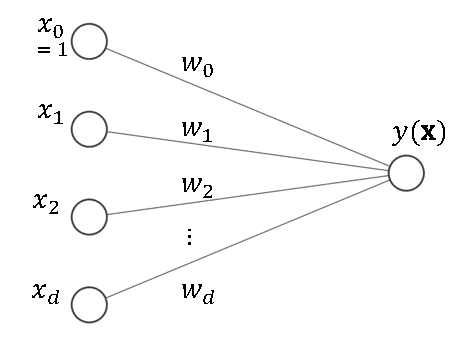
\includegraphics[width=\linewidth]{images/nn_perceptron.pdf}
        \caption{A computational graph of a standard perceptron. The input features $\mathbf{x}$ are linearly combined with the weights $\mathbf{w}$ and bias $w_0$ to produce the output $y$.}
        \label{fig:nn-perceptron}
    \end{subfigure}
    \hfill
    \begin{subfigure}[b]{0.45\linewidth}
        \centering
        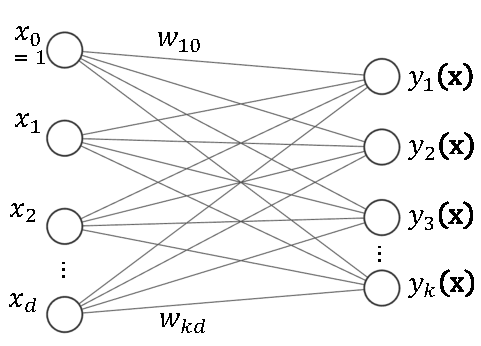
\includegraphics[width=\linewidth]{images/nn_multiclass.pdf}
        \caption{A computational graph of a multi-output perceptron. The input features $\mathbf{x}$ are linearly combined with the weights $\mathbf{w}$ to produce outputs $y_k$ for each dimension $k$.}
        \label{fig:nn-multiclass}
    \end{subfigure}
    \caption{Computational graphs for perceptron architectures. (a) Standard perceptron. (b) Multi-output perceptron.}
    \label{fig:nn-combined}
\end{figure}

\cref{eq:linear-regression} can be expressed as a computational graph, as shown in \cref{fig:nn-perceptron}. This architecture is commonly referred to as the standard perceptron, the simplest of neural networks.

\subsection{Generalization of Linear Models}
Linear regression can be extended to more complex settings, such as multi-output models (e.g.\ multi-class classification or multidimensional regression), with $y_k$ representing the output for the $k$-th dimension, and $x_0$ often set to $1$ as a convention for including the bias term $w_{k0}$:
\begin{equation}\label{eq:multi-output}
    y_k(\mathbf{x}) = \sum_{j=0}^{d} w_{kj} x_j
\end{equation}
Such an architecture is known as a single layer perceptron, and can be visualized as shown in \cref{fig:nn-multiclass}.

This can be further generalized by introducing non-linear basis functions $\phi_j(\mathbf{x})$, transforming the input features $\mathbf{x}$ before the linear combination:
\begin{equation}
    y(\mathbf{x}) = \sum_{j=0}^{d} w_j \phi_j(\mathbf{x})
\end{equation}
These non-linear transformations allow models to approximate non-linear relationships in data. Due to this, the loss can no longer be minimized in closed-form so iterative optimization algorithms such as gradient descent are used \cite{bishopPatternRecognitionMachine2006}.
Conventionally, these were basis functions were predefined and hand-crated based on domain knowledge, but we next look at deep learning models that can learn these basis functions.

\subsection{Deep Learning}
Multi-layer perceptrons build upon the foundations of linear models but eliminate the need to predefine input transformations. This is done by learning the parametrized basis functions from the data. 

One way to generalize the linear model is by applying a non-linear activation function $g$ to each input in \cref{eq:multi-output}. For example:
\begin{equation}
y_k(\mathbf{x}) = g\left(\sum_{j=0}^{d} w_{kj} x_j \right).
\end{equation}
To achieve this, neural networks add multiple layers to the computational graph, with each layer applying a linear transformation followed by a non-linear activation. A simple architecture is shown in \cref{fig:simple-nn-architecture} (with the addition of non-linearities), illustrating how the standard perceptron is extended to deeper networks.

Due to the non-linearities and layered structure, neural networks have high-capacity hypothesis spaces, suited to approximate the complex mappings such as multidimensional data such as images. 

\begin{figure}[h]
    \centering
    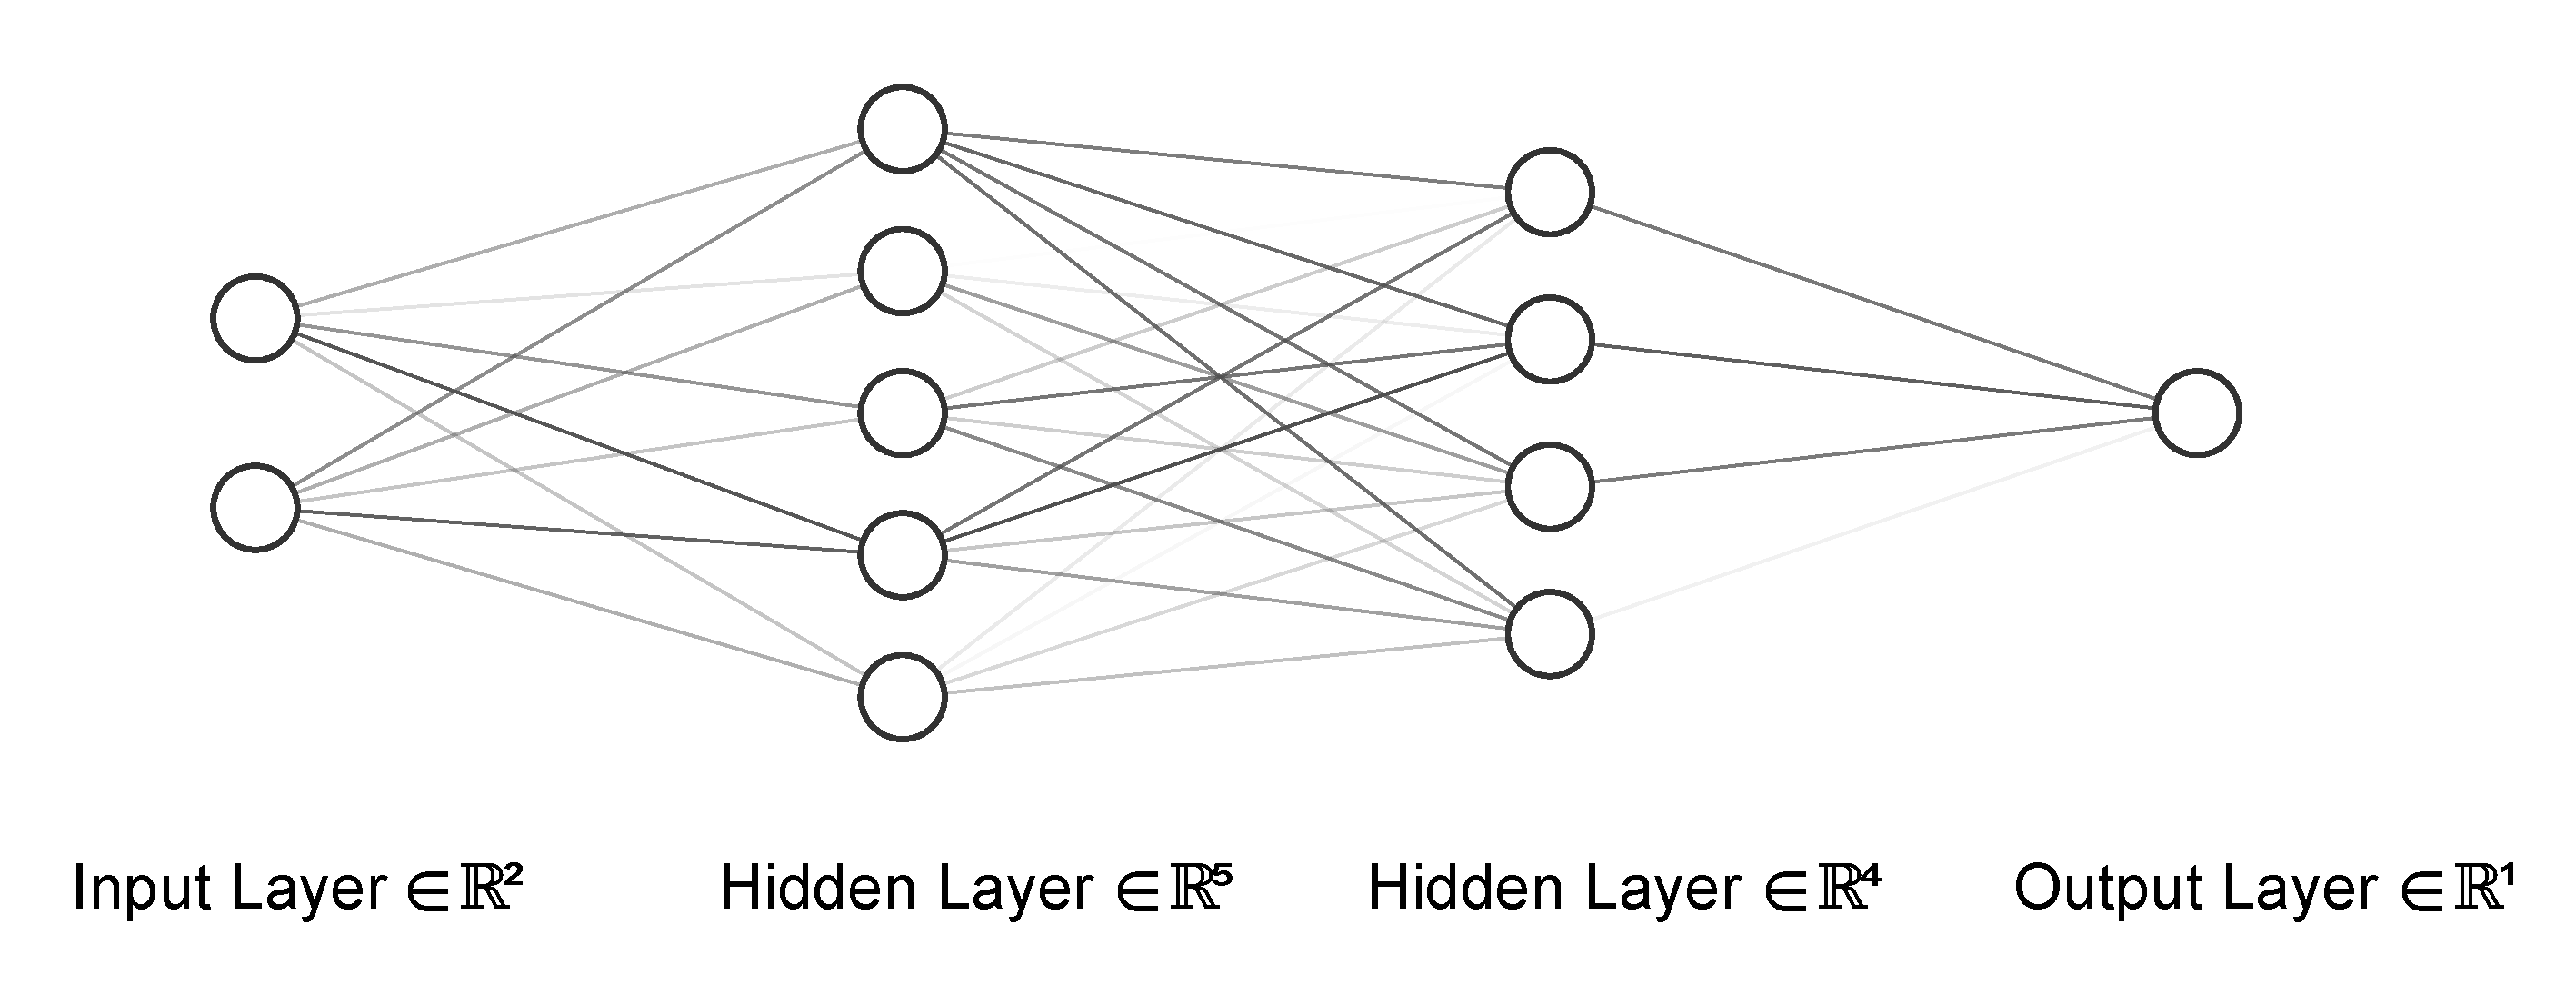
\includegraphics[width=1\linewidth]{images/simple_nn_architecture.pdf}
    \caption{An example trained fully connected neural network architecture with an input layer, two hidden layers, and an output layer. The input features are transformed through weights and biases, followed by a non-linear activation function in the first hidden layer. This process is repeated in the second hidden layer from outputs of the first (hidden) layer, producing the final outputs. The weights are represented by the lines connecting the neurons, with opacity indicating the weights' strength.}
    \label{fig:simple-nn-architecture}
\end{figure}

Activation functions are generally differentiable non-linear functions that introduce non-linearity into the network, allowing it to model complex relationships in the data. Common activation functions include the sigmoid function, that maps input values to a range between $0$ and $1$, useful to interpret probabilistically, and used in binary classification tasks. 
\begin{equation}
    S(x) = \frac{1}{1 + e^{-x}}
\end{equation}
Current state-of-the-art architectures often employ Rectified Linear Unit (ReLU) or its variants as the activation function, owing to their superior performance in training deep networks. ReLU defined as
\begin{equation}
    \text{ReLU}(x) = \max(0, x)
\end{equation}
sets negative inputs to zero while preserving positive inputs.

While ReLU is not differentiable at $x = 0$, it is widely favored due to its simplicity and effectiveness in training deep networks. Variants of ReLU, such as Leaky ReLU and Parametric ReLU have been introduced to address the issue of dead neurons, where neurons cease to learn during training. Leaky ReLU introduces a gradient for negative inputs
\begin{equation}\label{eq:leaky-relu}
    \text{Leaky ReLU}(x) = \max(\alpha x, x)
\end{equation}
defined by a small constant $\alpha$. Parametric ReLU extends this concept by allowing the gradient to be learned during training.

Training a neural network involves two primary phases: the forward pass and the backward pass. During the forward pass, the input data is propagated through the network, layer by layer, to generate an output. Following this, the backward pass occurs, in which the error, defined as the difference between the predicted output and the true output, is propagated back through the network using the gradient of the loss function. This step is crucial for updating the weights of the network.
The training process utilizes optimization algorithms, such as Stochastic Gradient Descent (SGD) \cite{sutskeverImportanceInitializationMomentum2013} or Adam Optimization \cite{kingmaAdamMethodStochastic2017}, which iteratively adjust the network's weights to reduce the loss.

\section{Neural Networks for Image Restoration using Noise2Noise Framework}
In the classical supervised-learning setting for image restoration, training assumes access to clean target images. Similar to \cref{sec:erm}, training can be formulated as
\begin{equation}
    \hat{h} = \argmin_{h \in \mathcal{H}} \frac{1}{\lvert \mathcal{S} \rvert} \sum_{(X, Y) \in \mathcal{S}} \ell(h(X; \theta), Y),
\end{equation}
where $\mathcal{S} \sim \mathcal{D}^n$ is the training set with images $\mathcal{S} = \{(X_1, Y_1), \dots, (X_n, Y_n)\}$ with $(X, Y)$  the noisy and clean target images.

Most often, instead of a multilayered perceptron architecture, \gls{CNN} are preferred for image restoration tasks. \gls{CNN} are well-suited for image data due to their ability to learn spatial hierarchies of features through convolution operations. he convolutional layers in a \gls{CNN} automatically detect patterns such as edges, textures, and shapes, while the pooling layers downsample the data to reduce both the number of parameters and computational complexity. The output of the convolutional layers, known as feature maps, captures these learned patterns, and max-pooling further enhances efficiency by retaining the most significant values in a region, reducing spatial dimensions. This pooling process also contributes to the network’s robustness to spatial variance. Furthermore, \glspl{CNN} impose a strong prior on the hypothesis space, assuming that the data is translationally invariant, which is a reasonable assumption for images \cite{goodfellowDeepLearning2016}. In the context of this work, we will explore a specific realization of \glspl{CNN}, namely the UNet, which is known for its effective use in image restoration tasks.

In many practical scenarios such as our \gls{MPES} data, obtaining the true clean image $Y$ is not feasible, although sufficiently high quality noisy data exists. In the instance when multiple noisy realizations of the same underlying signal are available, \citeauthor{lehtinenNoise2NoiseLearningImage2018} demonstrated that it is possible to train a neural network to learn a restoration mapping to the underlying clean signal using only noisy observations for both inputs and targets \cite{lehtinenNoise2NoiseLearningImage2018}, a framework known as \textit{Noise2Noise}. 

In the following sections, we see why Noise2Noise works and how it is applied to our image restoration problem.
\subsection{Point Estimation and Loss Functions}
We discussed in \cref{sec:generalization} that we aim to learn a hypothesis that generalizes to new data coming from the distribution $\mathcal{D}$. This can be done by minimizing the risk (\cref{eq:risk-min}). 

Consider an example point estimation problem where the objective is to find the scalar $\hat{x}$ that minimizes the expected deviation with respect to a set of observations $x_1, x_2, \dots, x_n$. This can be formalized as:
\begin{equation}
    \hat{x} = \argmin_{\hat{x}} \mathbb{E}[\ell(\hat{x}; x)]
\end{equation}
Different loss functions yield varying estimates based on the observations. For the case of $L_2$ loss, the minimization recovers the mean of the observations:
\begin{equation}\label{eq:l2-estimate}
    \hat{x} = \mathbb{E}[x]
\end{equation}
Similarly, for the $L_1$ loss, the estimate is the median of observations.

\subsection{Zero-Mean Noise}
Combining \cref{eq:risk} and \cref{eq:risk-min}, we can write the risk minimization problem as:
\begin{equation}
    \argmin_{h \in \mathcal{H}} \mathbb{E}_{x \sim \mathcal{D}} \left[\mathbb{E}_{y|x \sim \mathcal{D}} \left[ \ell(h(x; \theta), y) \right]\right]
\end{equation}
where using the law of total probability, the joint expectation $p(x,y)$ can be factorized to $p(x) \cdot p(y | x)$, and hence the expectation as well. This formulation is equivalent to solving the point estimation problem for each input sample separately. Due to this, the neural network inherits the properties of the loss function.

We established in \cref{eq:l2-estimate} that minimizing the $L_2$ loss recovers the mean of the observations. Now, consider the case where the training targets $y$ are corrupted with zero-mean noise, $\mathbb{E}[n] = 0$. The expectation remains unchanged i.e.\ $\mathbb{E}[y] = \mathbb{E}[x^\prime|y]$, with $x^\prime$ being the corrupted data. For example, we previously demonstrated Poisson noise being zero-mean  in \cref{sec:poisson-noise-model} (see \cref{eq:poisson-noise,eq:zero-mean-noise}), and hence, the $L_2$ loss could also recover, on expectation, the true value of a Poisson noise corrupted variable. Using other losses such as $L_1$ could allow recovery of signals with significant outlier content.

This principle can extend to neural network training as we already said that the network inherits the properties of the loss. When minimizing the risk, a neural network trained with zero-mean noise-corrupted targets will converge to the same optimal hypothesis as it would with clean targets. This holds true in the context of \gls{ERM} as well. With infinite training data, minimizing the empirical risk using noisy observations is mathematically equivalent to minimizing it with clean targets (\cref{eq:erm}).

\subsection{Noise2Noise Training for Finite Data}
Let us formalize the Noise2Noise training for a realistic case of finite examples. Consider a training set $\mathcal{S}^\prime = \{(X_1, X_1^\prime), \dots, (X_n, X_n^\prime)\}$ where $\mathcal{S}^\prime \sim \mathcal{D}^n$, each pair $(X, X^\prime)$ independent noisy realizations of the same underlying signal $y \sim \mathcal{D}$. Using the $L_2$ loss, we can redefine \gls{ERM} formulation from \cref{sec:erm} as
\begin{equation}\label{eq:erm-noise2noise}
    \hat{h} = \argmin_{h \in \mathcal{H}} \frac{1}{\lvert \mathcal{S^\prime} \rvert} \sum_{(X, X^\prime) \in \mathcal{S}^\prime} (h(X; \theta) - X^\prime)^2
\end{equation}
giving us a hypothesis $\hat{h}$ that minimizes the training error using only noisy observations for both inputs and targets.

For finite data, the quality of the estimate depends on the variance of the noise in the targets, divided by the number of samples $N$ \cite[supplementary~material]{lehtinenNoise2NoiseLearningImage2018}. This means that increasing the dataset size reduces the variance of the estimate, bringing it closer to the hypothesis had we minimized with clean targets. For image data, $N$ corresponds to the total number of scalar components\footnote{Number of images $n$ x number of voxels per image x number of color channels.} across the dataset, so having more voxels and data effectively brings us closer to the infinite data case.

\subsection{Regularization through Noisy Targets}
It is important to note that the earlier discussion assumed that learning with clean targets is inherently successful, while in fact, as we discussed before, \gls{ERM} is prone to overfit (generalizes poorly) in high-capacity hypothesis spaces. Using noisy targets actually has the unexpected benefit to act as a form of regularization. The noise in the targets perturbs the training objective, preventing the network from relying excessively on precise input-output mappings. For image restoration tasks, this can lead to better generalization, as the network focuses on recovering the underlying clean signal structure rather than spurious details in the data.

\section{Training an MPES Denoiser}
As seen in \cref{sec:image-formation}, the experimental setup (refer to \cref{section:hextof,section:dld}) for \gls{MPES} puts us in a unique position of having access to multiple noisy realizations of the same underlying image. This allows us to generate training data pairs where both the input and target are noisy versions of the same image. We can hence leverage the Noise2Noise \gls{ERM}, as shown in \cref{eq:erm-noise2noise}, to train a neural network to denoise \gls{MPES} images. We perform all the shown experiments with the $L_2$ loss\footnote{Some preliminary study using the $L_1$ loss also shows promise. This could be attributed to the significantly high noise at low count levels.} as the underlying images we aim to recover are the expectation of the noisy images.

Selecting the training data and neural network architecture are imperative for the success of the denoising task. Given the inherently multidimensional nature of \gls{MPES} data, it is advantageous to exploit cross-dimensional correlations to better estimate the underlying image. While 2D image restoration methods already utilize such principles in two dimensions, an example we already discussed with \gls{BM3D} in \cref{sec:bm3d}, higher dimensional data can provide additional information to improve the denoising performance\footnote{Algorithms such as BM4D \cite{maggionimNonlocalTransformdomainFilter} attempt to exploit this by considering the 3D structure of the data.}. 

This is further necessary since the 2D image slices from even our best dataset (\gls{ncounts} of \num{1.86e8} from \gls{GrIr}) are still noisy. In fact, in \cref{sec:mpes-bm3d-denoise}, we employed slice summing before denoising and also in evaluation. However, this summation leads to feature blurring and harnessing correlations across higher dimensions provides a more effective alternative.

To this end, we employ the UNET3D architecture, utilizing 3D convolutions, upsampling and pooling, instead of their 2D counterparts. In the following, we detail the data generation process, network architecture and the training and validation schemes.

\subsection{Training Data Generation}
\begin{figure}[h]
    \centering
    \begin{subfigure}[t]{0.59\linewidth}
        \centering
        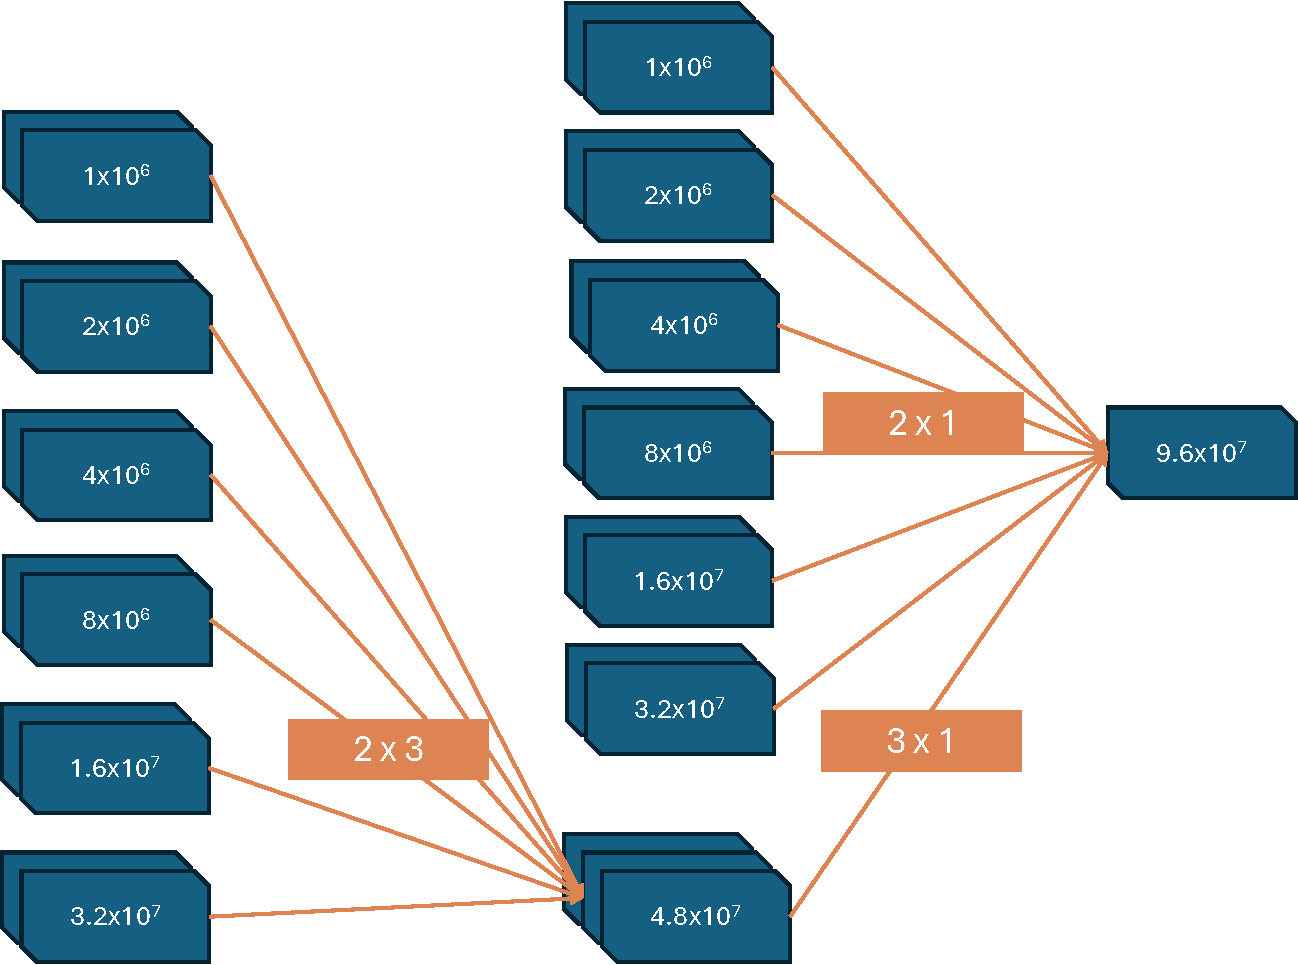
\includegraphics[width=1\linewidth]{images/training_flowchart.pdf}
        \caption{Flowchart illustrating the input-target dataset pairs, derived from subsets of the \gls{GrIr} dataset. A total of \num{34} unique noisy datasets are represented, with each dataset corresponding to one blue box in the chart. The different combinations shown in the chart generate \num{51} input-target pairs across counts \numrange{1e6}{9.6e7}.}
        \label{fig:training-data-flowchart}
    \end{subfigure}
    \hfill
    \begin{subfigure}[t]{0.39\linewidth}
        \centering
        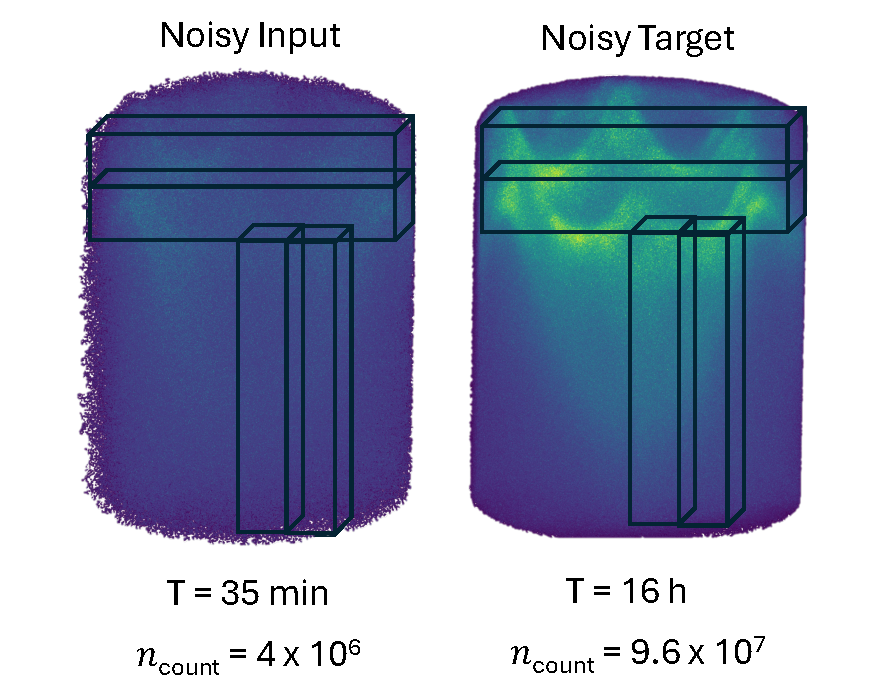
\includegraphics[width=1\linewidth]{images/training_3d_patch_example.pdf}
        \caption{Showing example noisy input and noisy target and how 3D subsets (also called patches) are extracted for training. On top, how extracted subsets could look.}
        \label{fig:training-3d-patch-example}
    \end{subfigure}
    \caption{Illustration of generating neural network training pairs. (a) The flowchart showing the input-target dataset pairs used for training, and (a) an example of noisy input and noisy target showing how 3D subsets are extracted from the volume. Through the combination with patch-based extraction, a total of \num{5967} training pairs are generated. The \num{4.8e7} and \num{9.6e7} counts serve as the target datasets, with \num{9.6e7} additionally functioning as the target for the \num{4.8e7} datasets.}
\end{figure}
The \gls{GrIr} dataset, with its high count, is used as the training dataset. While Noise2Noise training allows training with noisy data, it is not immediately apparent at what noise levels the training should be conducted. Naturally, the noise levels we aim to denoise should be reflected in the training set. Of particular interest are datasets obtained with shorter acquisition times $T$, and thus lower \gls{ncounts}. The authors in \cite{lehtinenNoise2NoiseLearningImage2018} demonstrated succesful training and inference on Poisson corrupted images with $\lambda \in [1, 50]$. Assuming Poisson noise\footnote{Which we know not to be the case from \cref{ch:pes-statistics}, but 
sufficies for the current argument.}, for our lowest-count noisy dataset, which has an average count per voxel of \num{5.98e-3}, and even our highest count dataset (\num{1.13} per voxel; see \cref{noisy-dataset-table}), the noise levels lie largely outside the range previously studied. Only the highest count dataset aligns with their researched range.

Hence, we go for the range that is most interesting for us, with inputs spanning \numrange{1e6}{4.8e7} and targets using \num{4.8e7} and \num{9.6e7}. To make this problem tractable and given the constraint of having independent datasets, a limited number (\num{34}) of input-target image pairs are used, as seen in \cref{fig:training-data-flowchart}. 

The ideal situation is if we have independent noisy dataset realizations. For instance, \num{1e6} \gls{ncounts} should not be sampled from the same region which is a subset of a \num{2e6} dataset, as overlapping events would introduce dependencies between datasets. While achieving complete independence is straightforward for lower-count datasets, it becomes increasingly challenging when sampling from the highest \gls{ncounts} of \num{1.86e8}. To mitigate this issue, we avoid using the maximum \gls{ncounts} during training, increasing the independence of datasets. 

Prior work by \citeauthor{lehtinenNoise2NoiseLearningImage2018} demonstrated that using cleaner targets, even with fewer noisy realizations (e.g., just two), significantly enhances denoising performance. Future improvements could involve incorporating other \gls{MPES} datasets to increase the pool of independent images. Additional studies could also examine whether including partially dependent datasets improves denoising performance.

We employ a patch-based approach to getting training pairs. Firstly, to increase the training data, having many independent training pairs, and secondly to make the problem computationally feasible, as training on entire 3D volumes would be prohibitively expensive, making batch-based training challenging. We extract 3D patches from the 3D volumes, as shown in \cref{fig:training-3d-patch-example}, generating \num{5967} training pairs. The patches are extracted at $60 \times 240 \times 240$ size, with a stride of $30 \times 120 \times 120$. The patches are then normalized to have zero mean and \numrange{-1}{1} ranges, common preprocessing step that centers the data and enhances neural network learning performance \cite{bishopDeepLearningFoundations2024}. 

To further augment the data, random rotations and flips are applied to the extracted patches. This augmentation not only increases the variability in the training data but also helps the neural network generalize better during inference.

\subsection{Model Architecture: UNET3D}
\begin{figure}
    \centering
    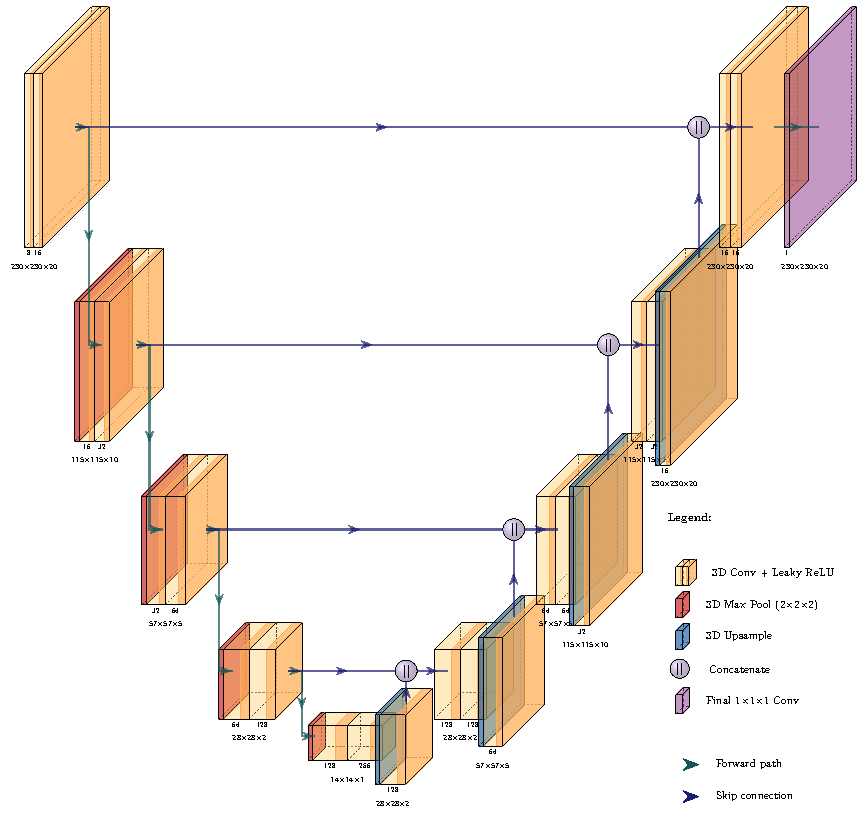
\includegraphics[width=0.8\linewidth]{images/unet_architecture.pdf}
    \caption{UNET3D architecture used for training the neural network, with example inputs propogated through the network. The architecture consists of an encoder-decoder structure with skip connections. The encoder compresses spatial information using a series of convolutional layers and 3D max-pooling operations, while the decoder reconstructs the data to its original dimensions using upsampling layers and convolutional operations. Skip connections link corresponding encoder and decoder levels, allowing feature reuse and aiding gradient flow during training.}
    \label{fig:unet-architecture}
\end{figure}

While in principle any denoising \gls{CNN} architecture could be used, we employ the UNET architecture, a popular choice for image restoration tasks, especially in medical imaging, where it has shown remarkable success \cite{ronnebergerUNetConvolutionalNetworks}. We extend the UNET architecture to train 3D data using 3D patches \cite{cicek3DUNetLearning2016}. Due to its relatively shallow architecture in comparison to deeper models, UNET accelerates the 3D learning process.

The name, UNET, takes after the architecture’s structure, a distinctive “U-shaped”, as illustrated in \cref{fig:unet-architecture}. UNET, similar to an autoencoder, consists of an encoder-decoder structure, forming the left and right halves of the “U-shape”. The difference from traditional autoencoders is the presence of skip connections (purple arrow) that link corresponding encoder and decoder levels. These connections allow the network to reuse features from the encoder during the decoding process, aiding gradient flow during training. The skip connections are also particularly useful in recovering fine-grained details lost during downsampling in the encoder.

The encoder compresses spatial information using a series of convolutional layers and 3D max-pooling operations. This progressively reduces the spatial dimensions while increasing the feature channels. On the other hand, the decoder reconstructs the data to its original dimension using upsampling layers and convolution operations. 

The model leverages 3D convolutions, allowing it to capture spatial features across the depth, height, and width dimensions simultaneously. Downsampling within the encoder is achieved through 3D max-pooling layers $2 \times 2 \times 2$ kernels, while the decoder employs 3D upsampling to restore spatial dimensions. The input data is processed in patches of size $60 \times 240 \times 240$ voxels\footnote{This is just how we train the data but \glspl{CNN} can process any arbitrary resolution, provided sufficient memory. In fact, during inference, we employ a larger patch size.}, which are reduced and then restored in the encoder-decoder pipeline. As illustrated in \cref{fig:unet-architecture}, intermediate feature maps progressively decrease in spatial dimensions (e.g., $230 \times 230 \times 20 \to 115 \times 115 \times 10 \to 57 \times 57 \times 5$) in the encoder and are restored in reverse order in the decoder. \todo{write about fmaps [16, 32, 64, 128, 256]}

The model uses Leaky ReLU activation functions, as seen in \cref{eq:leaky-relu}, with a negative slope of 0.01, which enhances gradient flow in regions with low activation values. Within each feature channel, group normalization (of size 8) is employed to improve training stability and performance. Group normalization performs normalization independent of the batch sizes by dividing the channels into groups and computing the mean and variance within each group across the channels. However, Batch Normalization calculates the mean and variance across the whole batch for every channel of features and is suited for larger batch sizes.

Additionally, due to memory limitations, we use a batch size of \num{16}. Hence, within each feature, group normalization (of size 8) is applied here instead, since batch normalization is known to be unstable, particularly for small batch sizes. Group normalization performs normalization independent of the batch sizes by dividing the channels into groups and computing the mean and variance within each group across the channels \cite{wuGroupNormalization2018}. However, Batch Normalization calculates the mean and variance across the whole batch for every channel of features and is suited for larger batch sizes.

The final layer of the network consists of a $1 \times 1 \times 1$ convolution, which maps the feature space to a single output channel, producing the denoised result.


\subsection{Training and Validation}
\begin{figure}
    \centering
    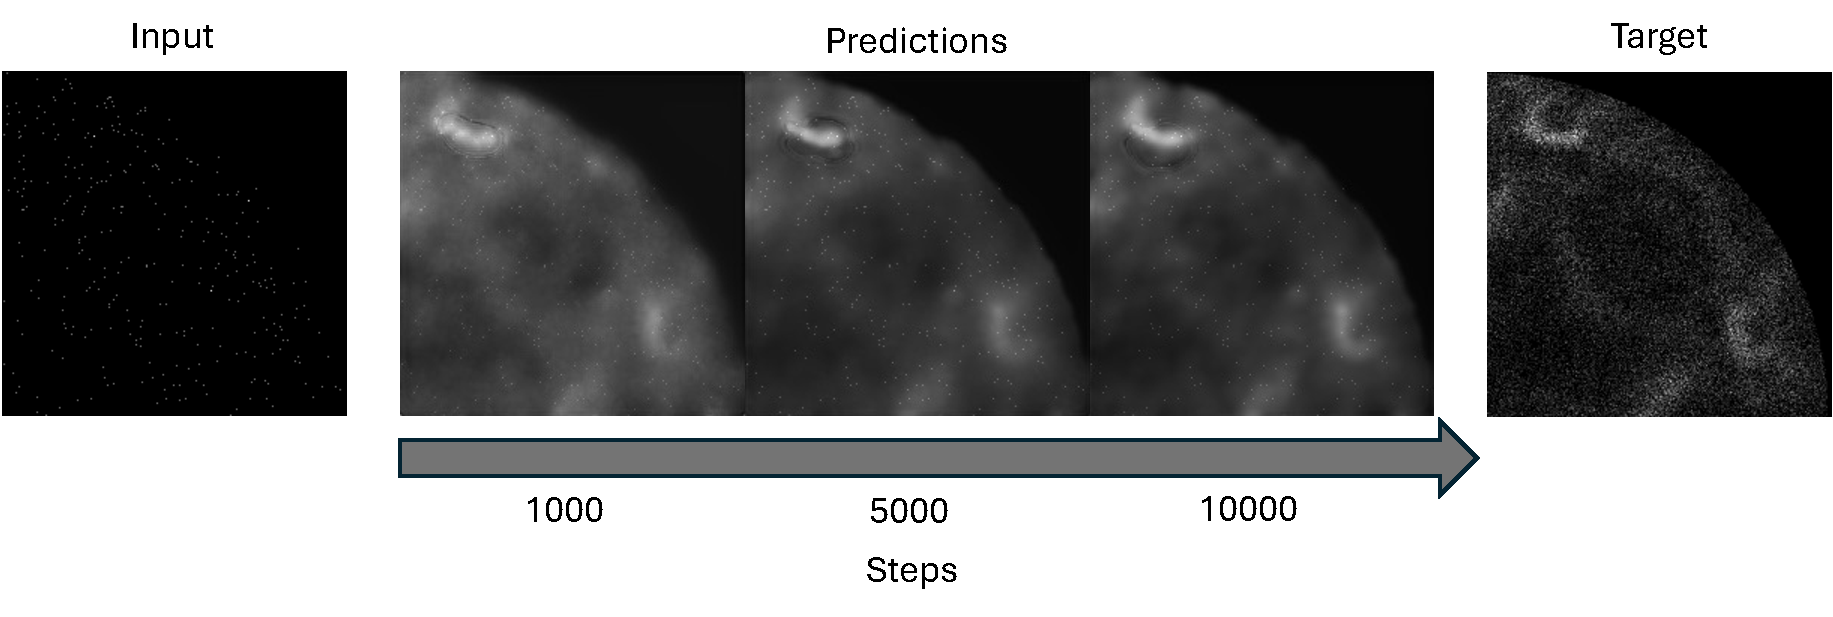
\includegraphics[width=1\linewidth]{images/training_progress_example2.pdf}
    \caption{Denoising predictions at step \numlist{1000;5000;10000} during training are shown, along with the input and target images. The key features, though blurry, are quickly discernible in the denoised images, even at early stages of training.}
    \label{fig:training-progress-example}
\end{figure}
For training, the model is optimized using the Adam optimizer with an initial learning rate of \num{0.001} and beta values of \num{0.9} and \num{0.99}. The learning rate is adjusted dynamically using a \texttt{ReduceLROnPlateau} scheduler, which reduces the rate by a factor of \num{0.1} if the primary evaluation metric does not improve for \num{10} validation runs. The training is conducted with a batch size of \num{16}, for a maximum of \num{1e3} epochs or until \num{1e5} iterations are completed. Validation is performed every \num{1e3} iterations using \gls{SSIM} as the primary metric and \gls{PSNR} as evaluation metrics. This training was performed prior to the results regarding \gls{MSSSIM} in \cref{sec:metric_comparison_experiment}. Therefore, while \gls{SSIM} was used here, a better validation could be obtained using \gls{MSSSIM} in future work.

For validation, we split our 3D dataset with a 80-20 ratio along the $E$ dimension, with the first 80\% used for training and the remaining 20\% for validation. Most of the key features exist in the training set but due to limited data availability, we can only employ low quality features for validation. We use the highest count dataset to validate against. The validation set is used to monitor the model's performance and prevent overfitting. 

Checkpoints are saved after every validation run, enabling resumption from the last checkpoint if interrupted. Furthermore, the model with the best validation \gls{SSIM} score is saved separately. The training progress for a single (training) example is shown in \cref{fig:training-progress-example}, where the denoising performance shows perceptually significant improvements already at early stages of training.



\begin{figure}
    \centering
    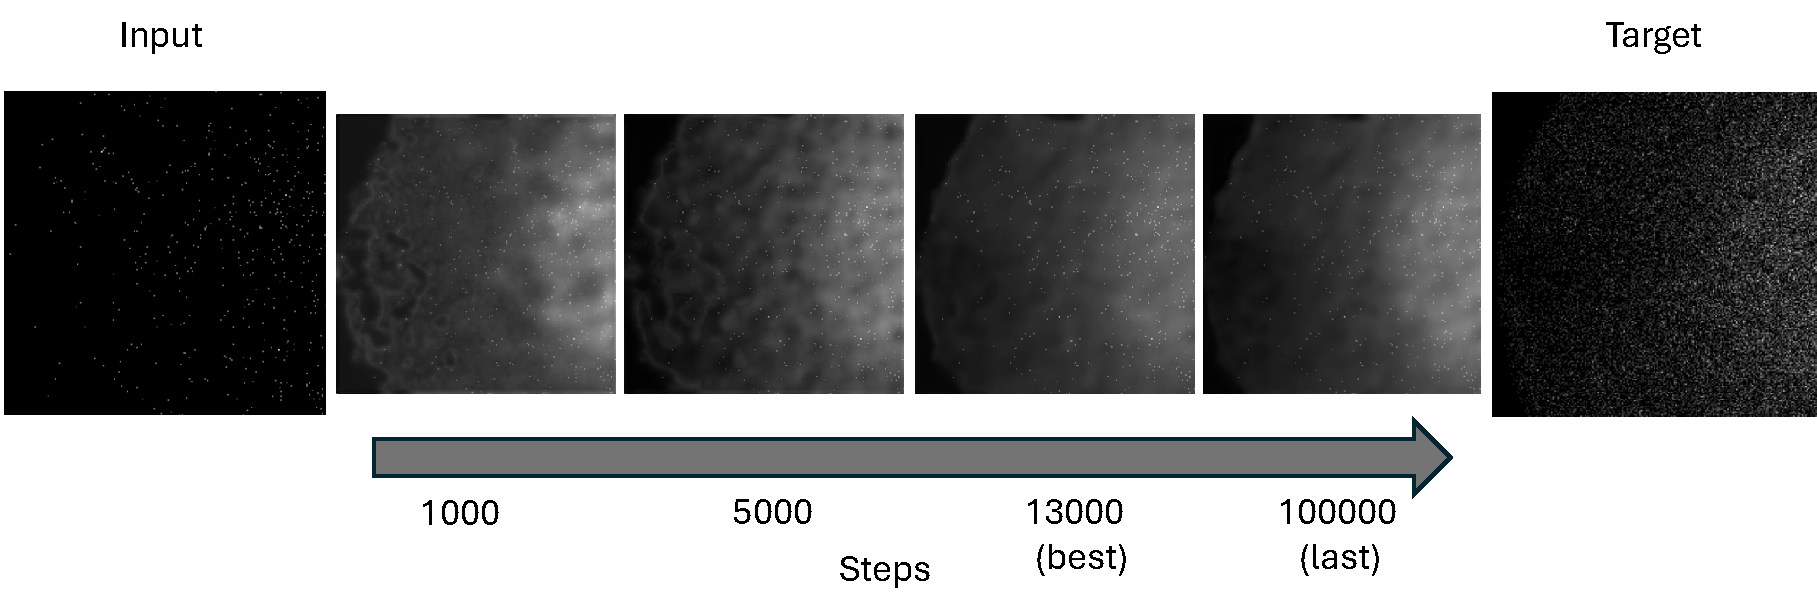
\includegraphics[width=1\linewidth]{images/val_over_time.pdf}
    \caption{Denoising predictions at step \numlist{1000;5000;13000;100000} during validation are shown, the latter two of which correspond to the best and last models. The input and target images are also shown. The validation set features not as discernible as the training set, as they correspond to energies much above the Fermi level.}
    \label{fig:val-progress-example}
\end{figure}

The training and validation loss are shown in \cref{fig:loss-training-val}. It has already been exemplified in \cite{lehtinenNoise2NoiseLearningImage2018} that the training loss does not decrease during training, as the network can not possibly learn to transform one instance of noise to another, as the training asks for the impossible. Hence, other than the initial decrease, the network loss stays plateaued consistently across \num{1e5} steps. However, since our validation target is a higher quality noisy dataset \num{1.86e8}, the expectation would be that it reports higher loss values. But as we discussed earlier, the validation set data is much above Fermi level, with features indistinguishable. The validation loss can be seen to converge to a stable value at \num{4e4} steps. 

\begin{figure}
    \centering
    \begin{subfigure}[t]{0.49\linewidth}
        \centering
        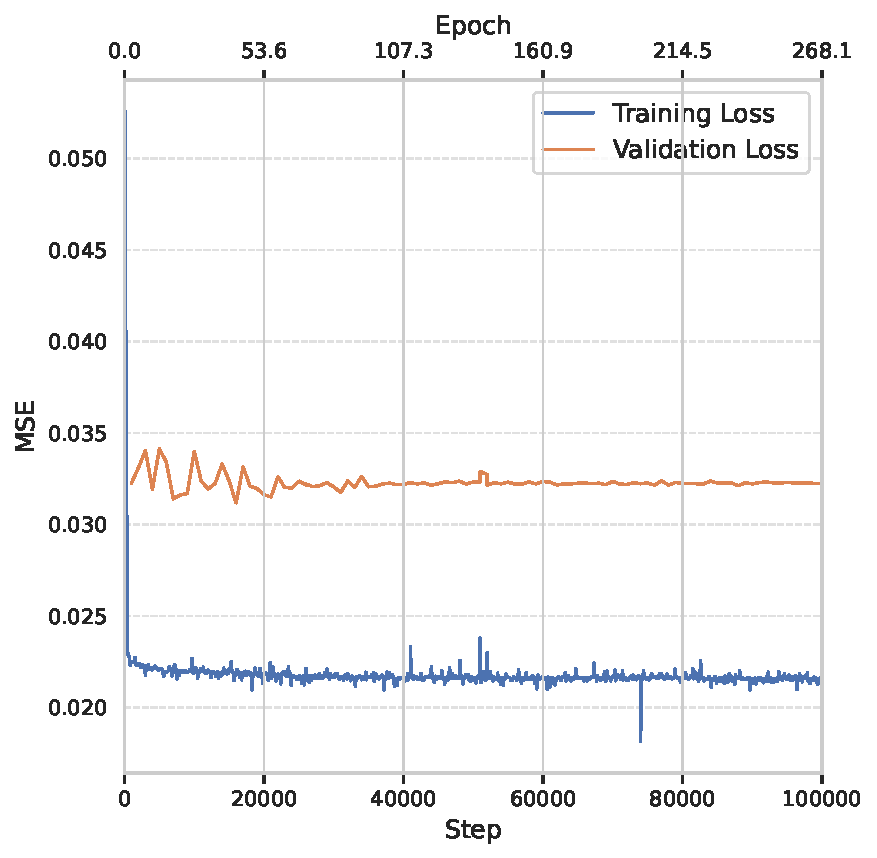
\includegraphics[width=1\linewidth]{images/loss_training_val.pdf}
        \caption{Training and validation loss. The gap exists due to the validation set being compared with higher quality targets. The validation loss converges to a stable value at \num{4e4} steps.}
        \label{fig:loss-training-val}
    \end{subfigure}
    \hfill
    \begin{subfigure}[t]{0.49\linewidth}
        \centering
        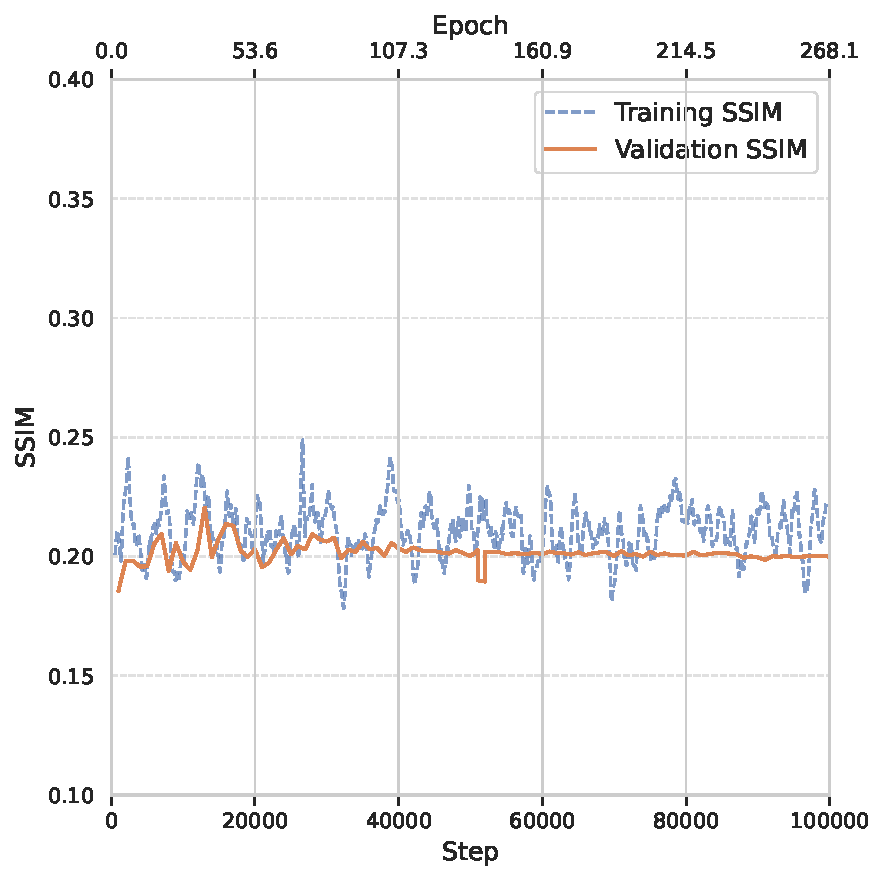
\includegraphics[width=1\linewidth]{images/ssim_training_val.pdf}
        \caption{\gls{SSIM} scores across training and validation. The scores show constant fluctuations around an average value during training but show less fluctuations during validation, where validation also converges to a stable value at \num{4e4} steps.}
        \label{fig:ssim-training-val}
    \end{subfigure}
    \caption{(a) Training and validation loss and (b) \gls{SSIM} scores over training steps and epochs. The UNET3D architecture is trained, using noisy input-targets pairs.}
    \label{fig:loss-ssim-training-val}
\end{figure}

The metric assessment using \gls{SSIM}, shown in \cref{fig:ssim-training-val}, also shows constant fluctuations around an average value in during training but are shown to be converging in the validation. We therefore look at two models, the (\textit{best}) model with the highest validation \gls{SSIM} of \num{0.23} that happens early on during training, after about \num{25} epochs\footnote{Meaning we do \num{25} passes of our entire dataset during training.}, and the (\textit{last}) model at end of training, where the validation \gls{SSIM} has converged to \num{0.2}.

\begin{figure}
    \centering
    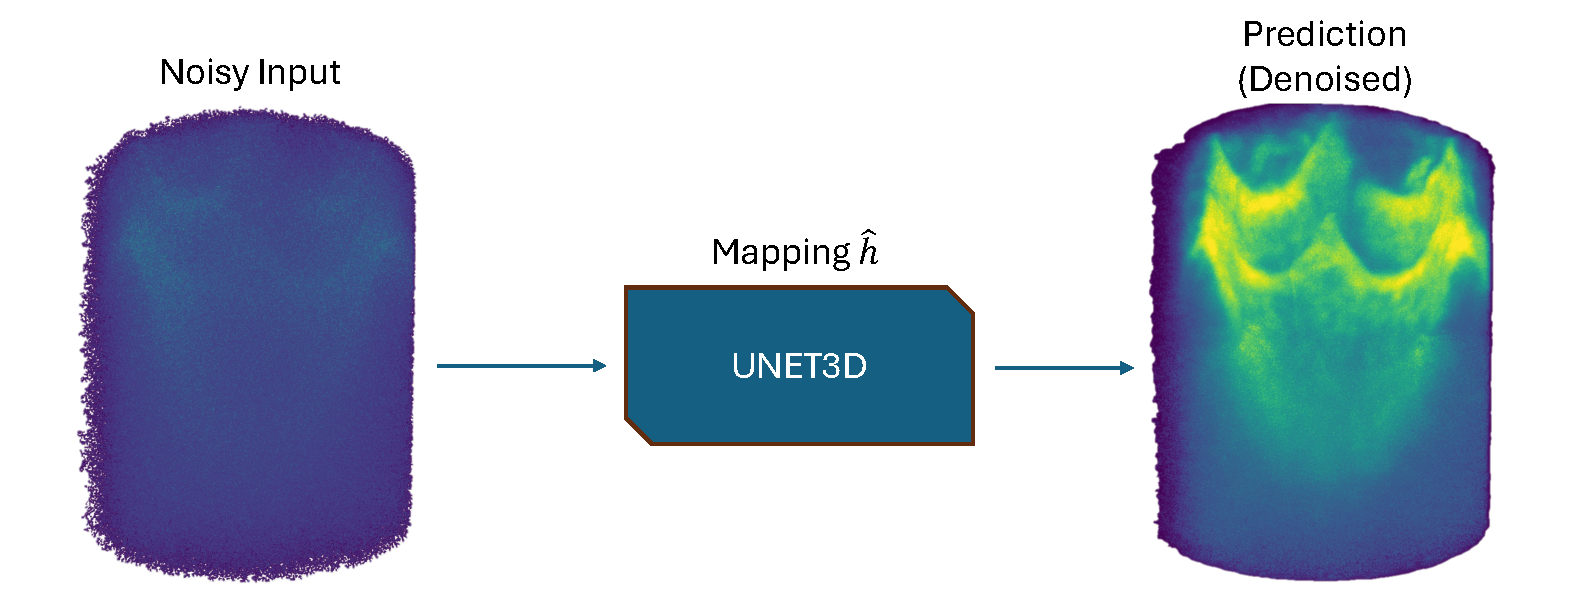
\includegraphics[width=1\linewidth]{images/noisy_denoised_3d.pdf}
    \caption{Example prediction (forward pass) from \num{4e6} count dataset, using the best model The prediction resolves the key features in the noisy input, showing the effectiveness of the denoising model.}
    \label{fig:3d-image-noisy-denoised-training}
\end{figure}

\begin{figure}
    \centering
    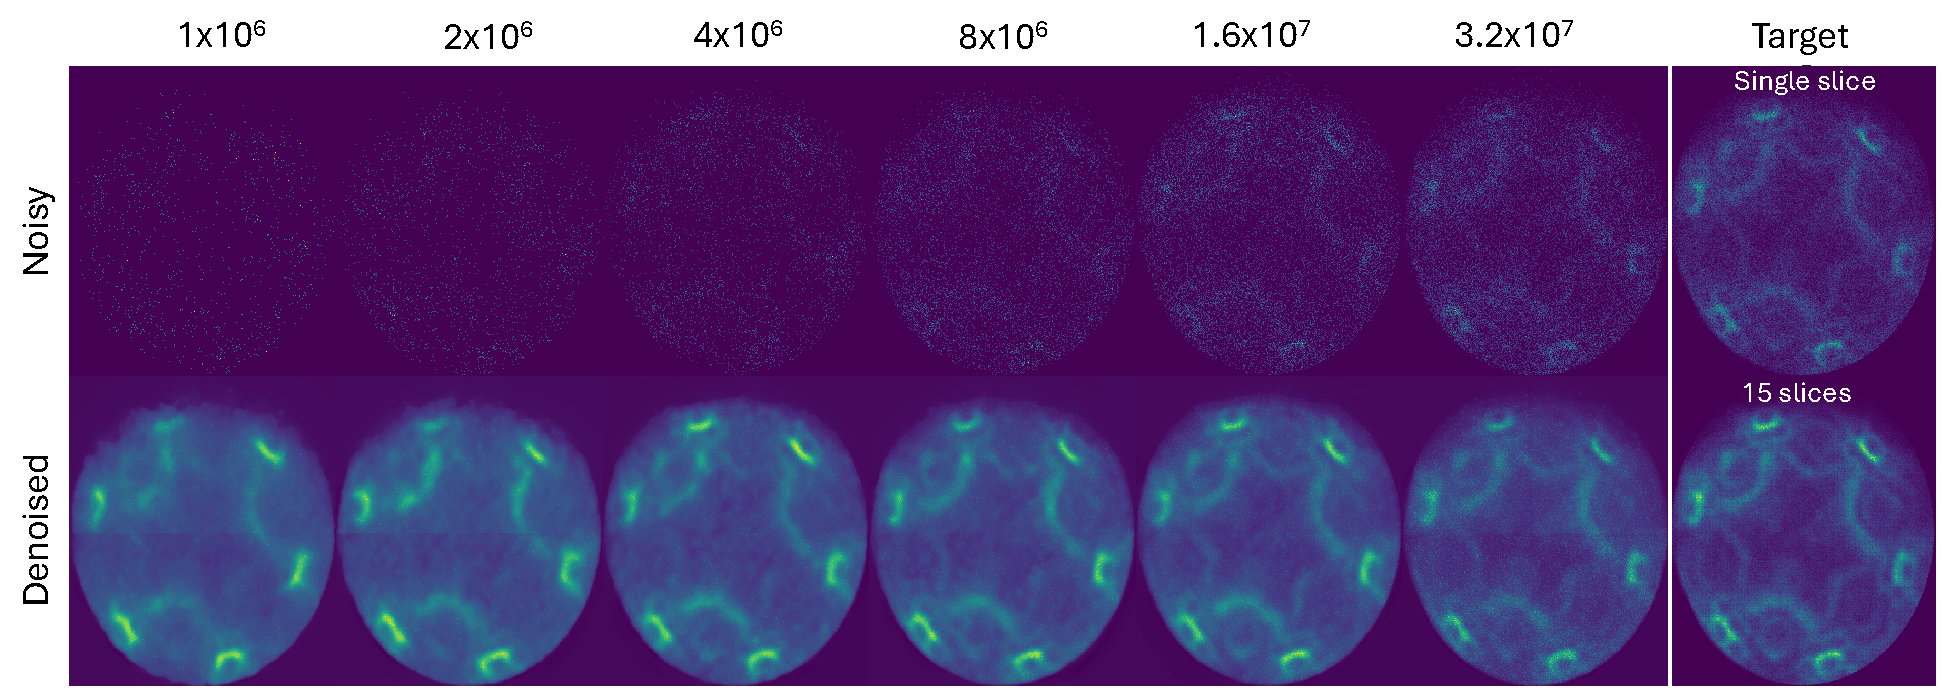
\includegraphics[width=1\linewidth]{images/images_noisy_denoised_with_target.pdf}
    \caption{Noisy and denoised \gls{ky}-\gls{kx} cuts with window size $w=1$ shown for \gls{GrIr} dataset. Each column corresponds to \numlist{1e6;2e6;4e6;8e6;1.6e7;3.2e7;1.86e8} counts, respectively; where the last column is the target image with $w=1$ in row 1 and $w=15$ in row 2. Below \num{8e6} counts, none of the features are discernible for noisy images, while the denoised images show clear features similar to the target.}
    \label{fig:images-noisy-denoised-training}
\end{figure}

\cref{fig:3d-image-noisy-denoised-training} illustrates how the mapping $\hat{h}$ learned during training predicts data. Looking at \cref{fig:images-noisy-denoised-training}, we see the noisy and denoised \gls{ky}-\gls{kx} cuts for the \gls{GrIr} dataset, at different noise (count) levels. The noisy images show no discernible features below \num{8e6} counts, while the denoised images show clear features similar to the target. The model evaluated on the training set hence shows promising results. To really be sure that the model achieved generalized capability of denoising the experimental data, and not just learned the features of the training set, we need to evaluate it on independent test data.



\subsection{Evaluating Model Denoising Performance}
\begin{figure}
    \centering
    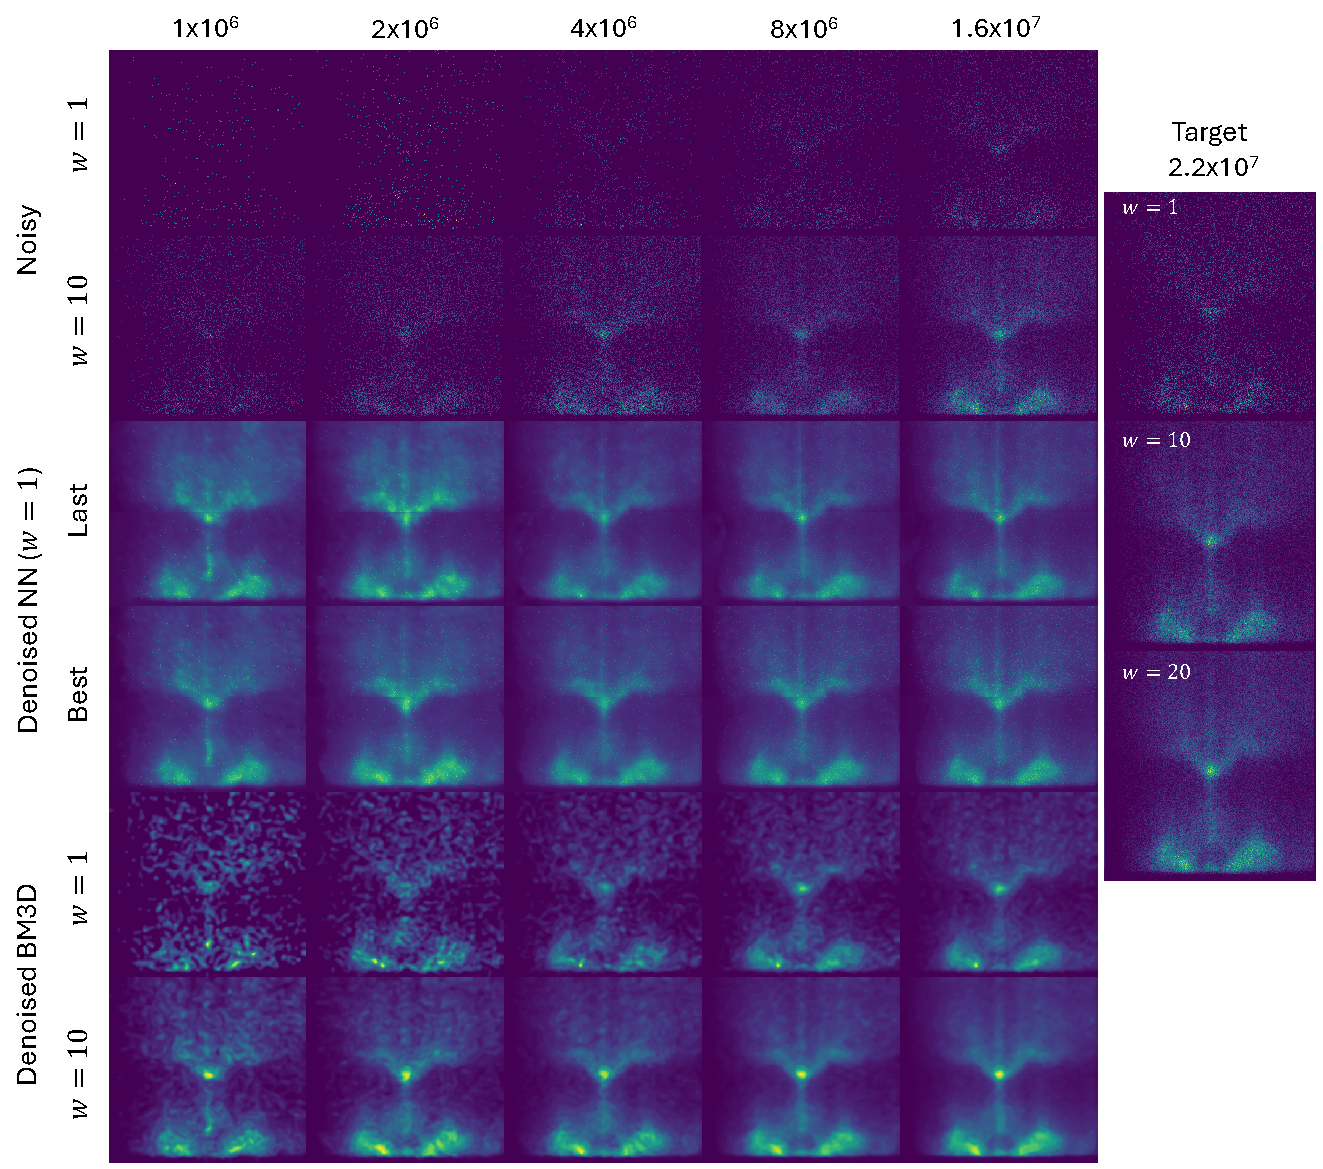
\includegraphics[width=1\linewidth]{images/nn_denoised_counts_best_last_ex_bm3d.pdf}
    \caption{Comparison of \gls{kx}–\gls{E} slices for various \gls{ncounts}. The target image is shown for a single slice and for slice-summed images with \gls{winsize} values of \num{10} and \num{20}, demonstrating the effect of summing slices for visual quality improvement. The noisy image is also depicted as a slice-summed result, emphasizing that slice summing acts as a basic form of noise reduction. Denoised results are shown for the best and last trained neural network models ($w=1$), alongside \gls{BM3D}–Anscombe denoising applied with the optimal parameter $\sigma_{\text{o}}$ for $w=10$ and the same parameter used for $w=1$. The results illustrate that the neural network outperforms BM3D–Anscombe denoising at lower counts (\num{1e6}). At higher counts and when slices are summed, BM3D’s performance improves relative to the neural network.}
    \label{fig:nn-denoised-counts-best-last-ex-bm3d}
\end{figure}

We use the \gls{GdW} dataset for evaluating the model's generalization capability. \cref{fig:nn-denoised-counts-best-last-ex-bm3d} shows a \gls{kx}--\gls{E} slice for noisy and denoised images for best and last models, as well as comparison with \gls{BM3D}--Anscombe denoising. The plot also show the slice summed image with \gls{winsize} of \num{10} for noisy image, that also acts as some sort of denoising. BM3D results are also shown for this sum as for lower counts, BM3D performs poorly. \cref{fig:nn-denoised-counts-best-last-xy-bm3d} shows the \gls{ky}--\gls{kx} slice for the same models and \gls{BM3D}--Anscombe denoising.

From this it can be understood that neural network based denoising performs much better at lower counts (even at \num{1e6}) than BM3D based denoising. At higher counts and summed slices, the BM3D denoising also perform well, a conclusion we already drew in \cref{ch:datasets_bm3d}. To see if slice summing has any improvement in denoising performance of the neural network, one can look at  \cref{fig:nn-denoised-counts-best-last-xy-bm3d-slice-sum-last-model}, showing the last model denoising performance on the summed slice. The denoising performance is not improved by the slice summing, as the features are already well resolved in the individual slices. As before, this leads to feature blurring and for the neural network model, is not leading to any significant perceptual improvement. This can be explained by the fact that my using a 3D model, we have already taken into account the correlations across the depth dimension, and hence the slice summing does not provide any additional information.

\begin{figure}
    \centering
    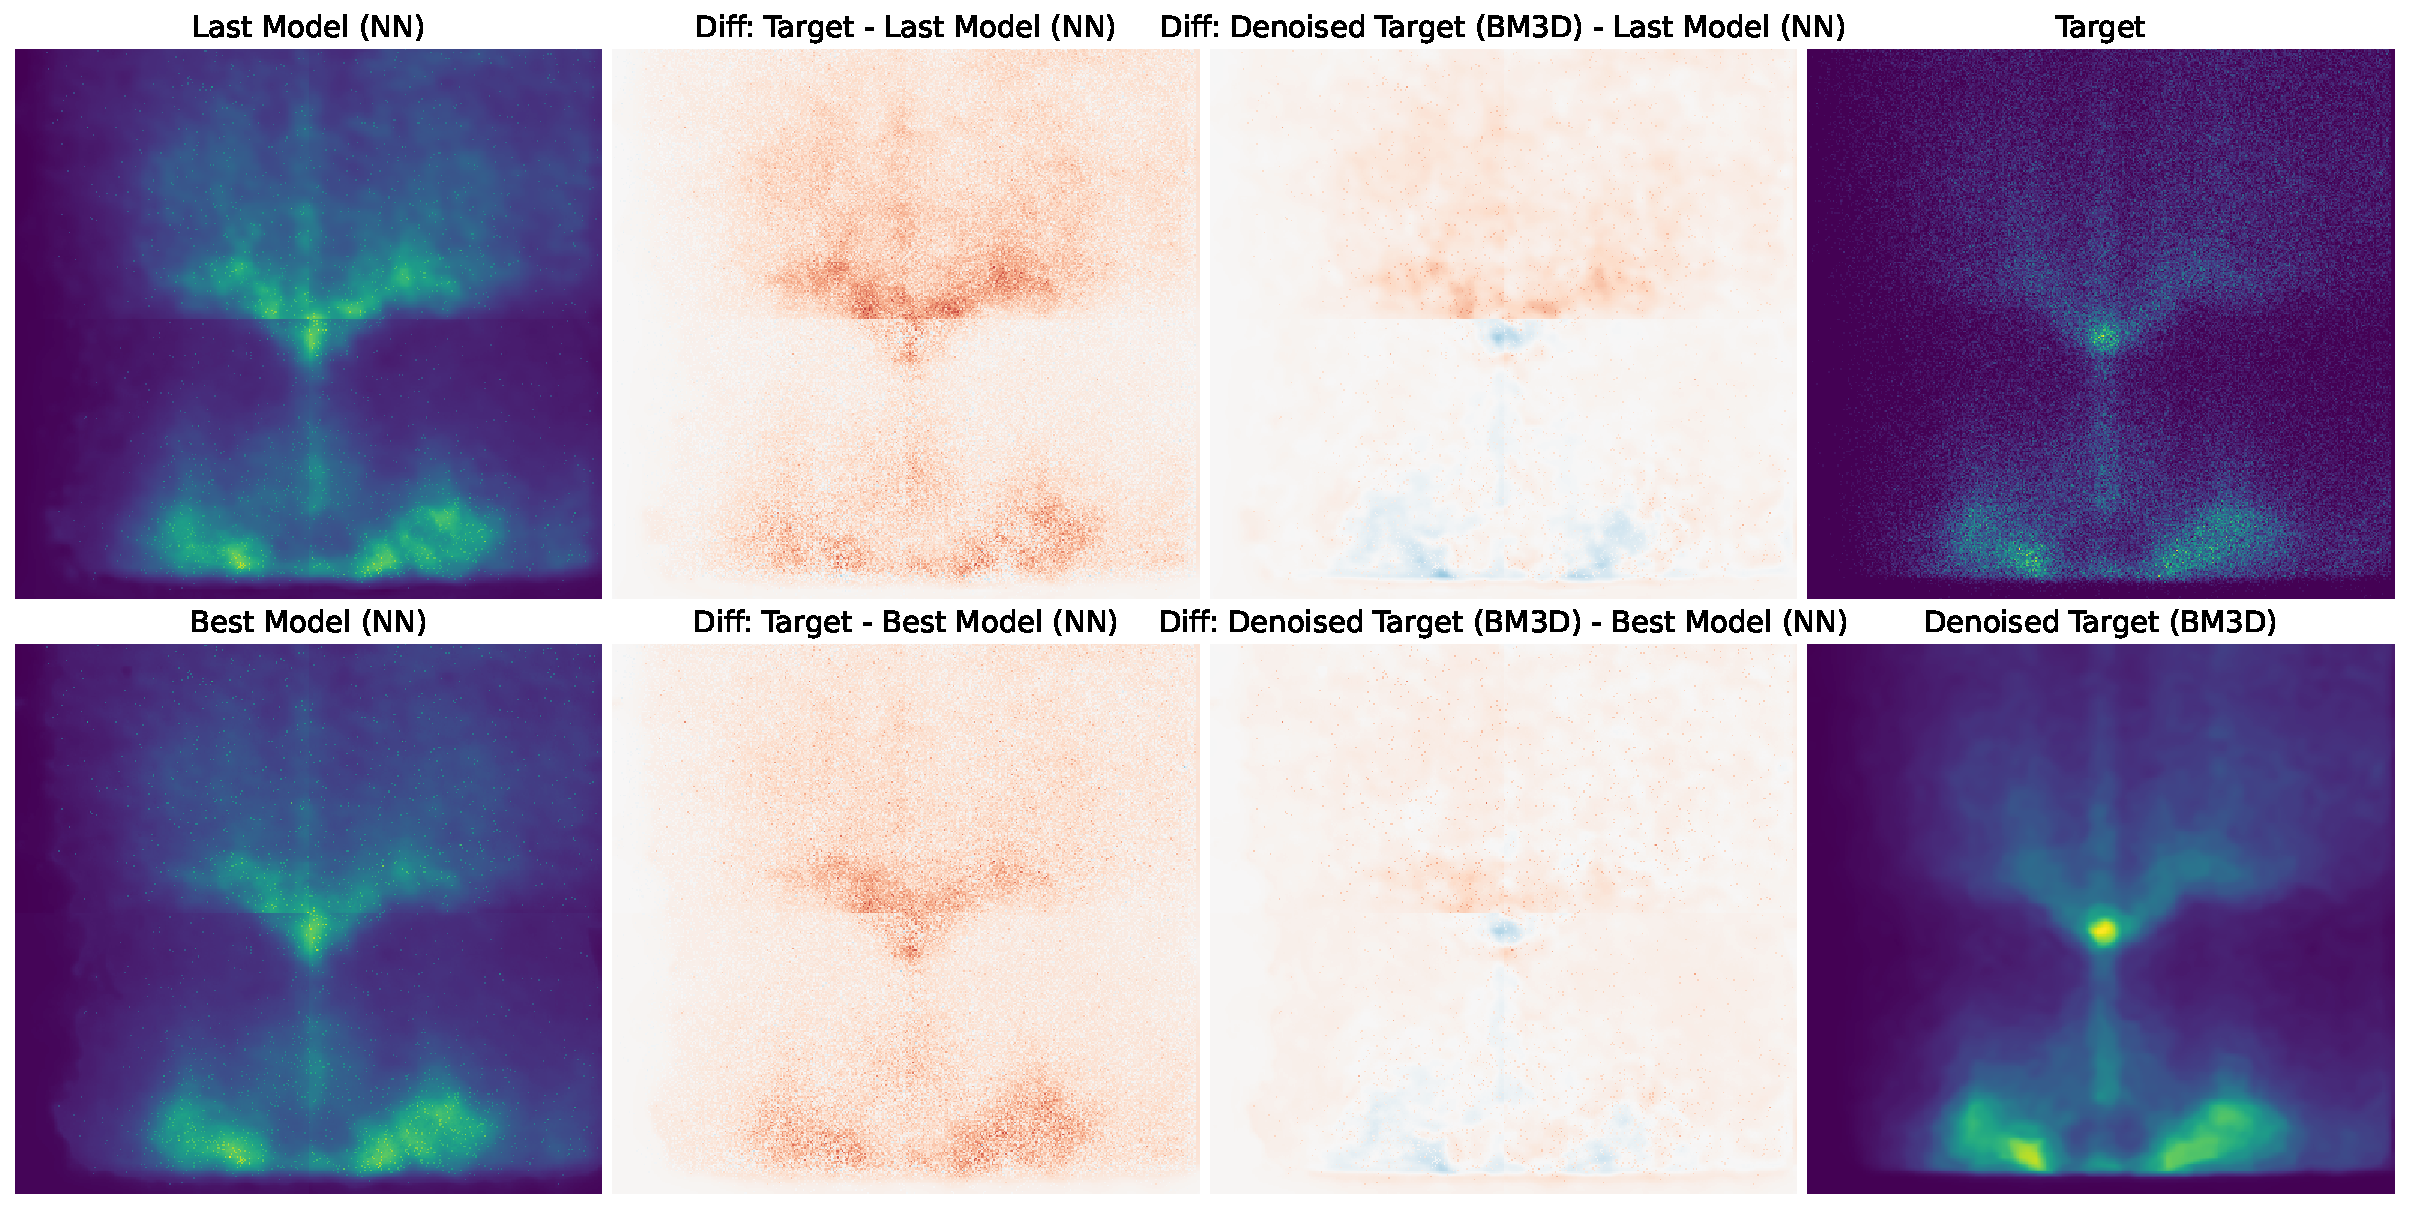
\includegraphics[width=1\linewidth]{images/nn_diff_plots_2M.pdf}
    \caption{Difference images comparing the best and last models for \gls{ncounts} \num{2e6}. The differences are computed relative to two references: the slice-summed target image with \gls{winsize} of \num{10}, and its BM3D-denoised version. The red regions indicate where the prediction is brighter than the noisy target, while blue regions indicate where the target is brighter. The target itself is noisy, so when subtracting the denoised outputs from the target, mostly red regions are visible. However, when using the BM3D-denoised target as a reference (assumed to approximate the correct image), the differences are mostly white (close to 0), with some blue regions where predicted features are less intense compared to the reference. These difference plots highlight that the best model preserves features more effectively and aligns better with the BM3D-denoised target compared to the last model.}
    \label{fig:nn_diff_plots_2M} 
\end{figure}

Let us now explore whether the longer training time to obtain the last model is worthwhile, since the best model is obtained early on. To explore this,  we can look at the difference images between the predicted output and target image. Since the target is noisy, we look at slice summed images with \gls{winsize} of \num{10} to get a better idea of the features. Furthermore, we also compare the best and last models with a BM3D denoised target image. Since BM3D is performing well at these counts, it can be used as a reference for the neural network denoising performance.

The difference images are shown in \cref{fig:nn_diff_plots_2M} and \cref{fig:nn_diff_plots_8M} for \num{2e6} and \num{8e6} counts, respectively. Comparing with the target, both models show unsharp features at \cref{fig:nn_diff_plots_2M}, especially the last model. Whereas, \cref{fig:nn_diff_plots_8M} approaches much closer to the target looking at the difference images. Perceptually, the last model has features slightly better resolved but in this. When looking at \gls{MSSSIM} scores, the best models report better values for lower counts (e.g.\ best \num{0.68} vs.\ last \num{0.65} with \num{2e6} and both best and last with \num{0.73} at \num{8e6}) and converges with last model for higher counts. Since we are especially interested in lower counts denoising, it is not clear if the longer training time is justified, and further investigation is needed. It should be noted that the target image is not as representative of clean target with only count \gls{ncounts} of \num{2.21e7} compared to the \gls{GrIr} target of \num{1.86e8}.

\begin{figure}
    \centering
    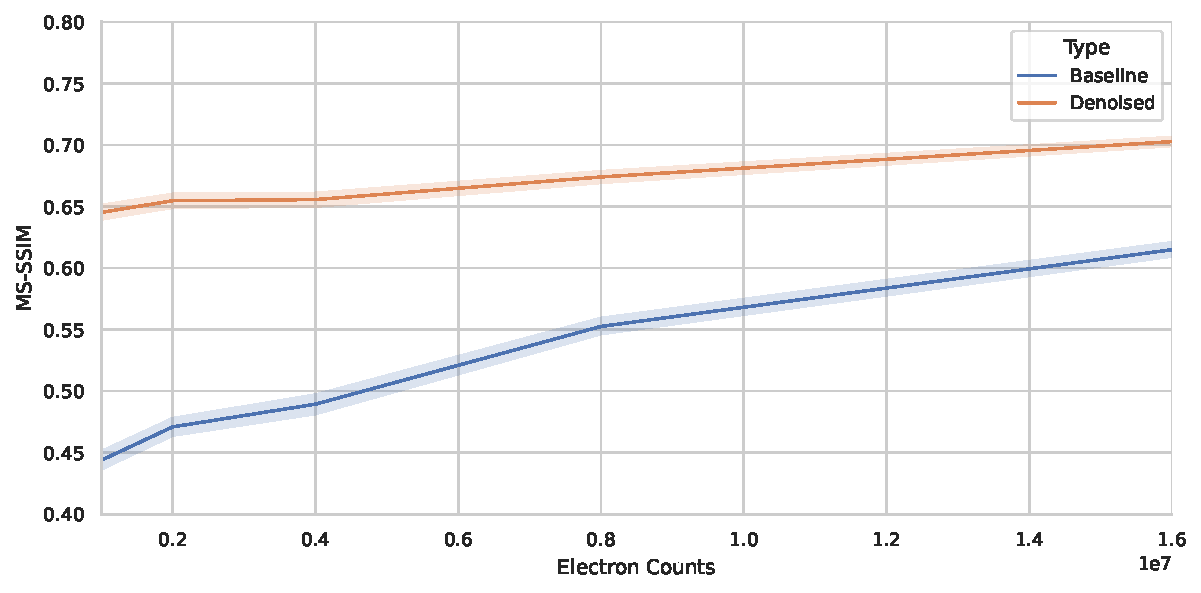
\includegraphics[width=1\linewidth]{images/nn_gdw_msssim.pdf}
    \caption{Denoising performance of (best) neural network as a function of \gls{ncounts}, measured using \gls{MSSSIM}. The comparison is done with slice-summed target with $w=10$. The baseline metric is computed using the noisy image as input. Different from \gls{BM3D}, the neural network denoising performance stays relatively consistent across the \gls{ncounts}, and is especially effective at lower counts.}
    \label{fig:gdw-test-metirc}
\end{figure}


At the end, we can look how the \gls{MSSSIM} scores improve with increasing counts, similar to how it is done with BM3D in \cref{fig:bm3d-msssim}. We have only looked at the best model but the same could be done for the last model. The \gls{MSSSIM} scores are shown in \cref{fig:gdw-test-metirc}, where the comparison is done between single slice denoised images with a slice summed target image ($w=10$). Perceptually (see \cref{fig:nn-denoised-counts-best-last-xy-bm3d-slice-sum-last-model}) the denoising performance with neural network far exceeds that of BM3D at low counts, even when denoising slice summed images with BM3D. The neural network denoising performance is also better than BM3D at higher counts for single slices, but the slice summed images and high counts ($geq \num{8e6}$) is just as good, or better. We do not discuss the \gls{MSSSIM} scores in detail, as the perceptual results are more important, and the \gls{MSSSIM} scores are consistent with the perceptual results.



% \begin{figure}
%     \centering
%     \begin{subfigure}[b]{1\linewidth}
%         \centering
%         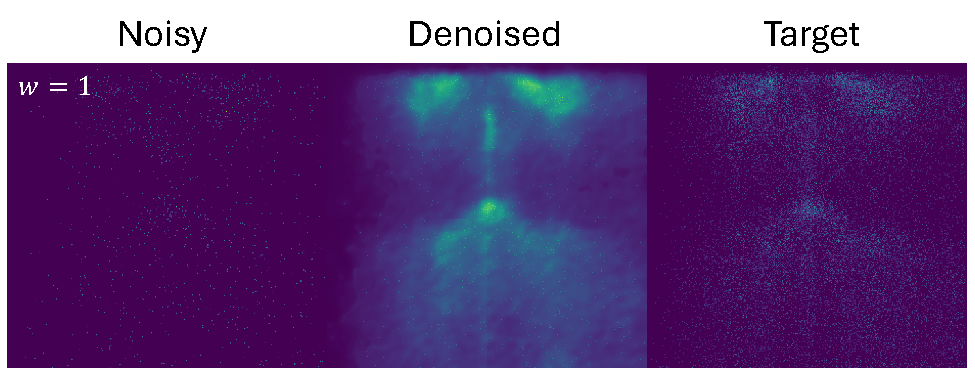
\includegraphics[width=1\linewidth]{images/nn_denoised_ex_w_1.pdf}
%         \caption{}
%         \label{fig:nn-denoised-ex-w-1}
%     \end{subfigure}

%     \begin{subfigure}[b]{1\linewidth}
%         \centering
%         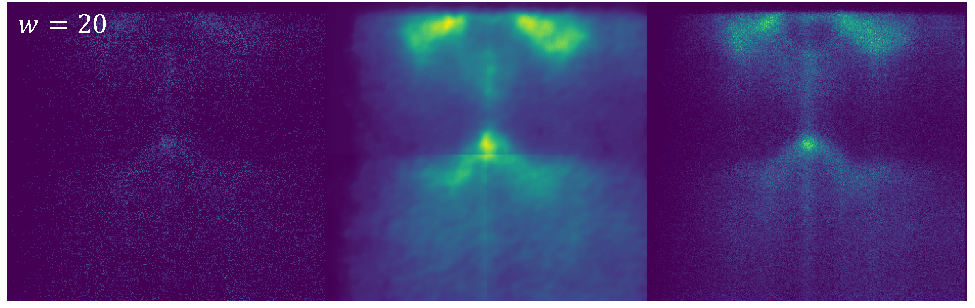
\includegraphics[width=1\linewidth]{images/nn_denoised_ex_w_20.pdf}
%         \caption{\num{4e6} count dataset. The denoising performance leaves room for improvement, using the adjusted optimal $\sigma_{\text{o}}\approx0.4$.}
%         \label{fig:nn-denoised-ex-w-20}
%     \end{subfigure}
%     \caption{}
%     \label{fig:nn-denoised-ex-w}
% \end{figure}

% \begin{figure}
%     \centering
%     \begin{subfigure}[b]{1\linewidth}
%         \centering
%         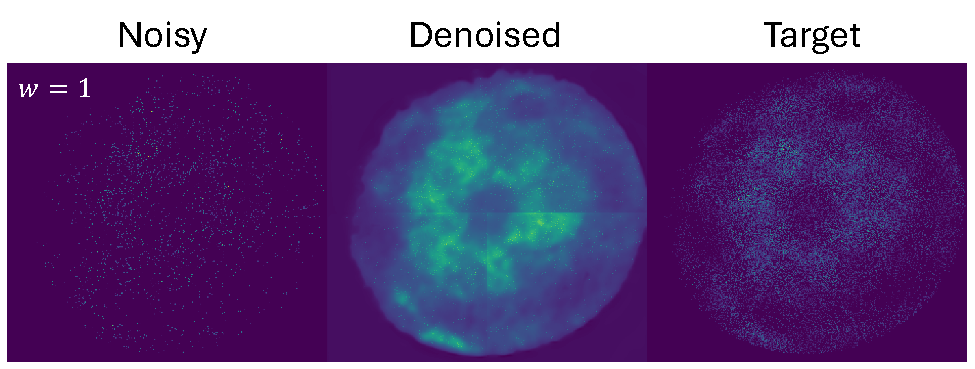
\includegraphics[width=1\linewidth]{images/nn_denoised_xy_w_1.pdf}
%         \caption{}
%         \label{fig:nn-denoised-xy-w-1}
%     \end{subfigure}

%     \begin{subfigure}[b]{1\linewidth}
%         \centering
%         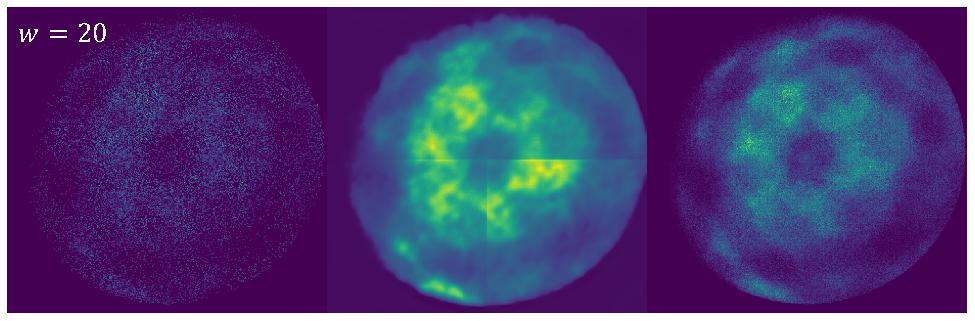
\includegraphics[width=1\linewidth]{images/nn_denoised_xy_w_20.pdf}
%         \caption{}
%         \label{fig:nn-denoised-xy-w-20}
%     \end{subfigure}
%     \caption{}
%     \label{fig:nn-denoised-xy-w}
% \end{figure}


% \begin{figure}[h]
%     \centering
%     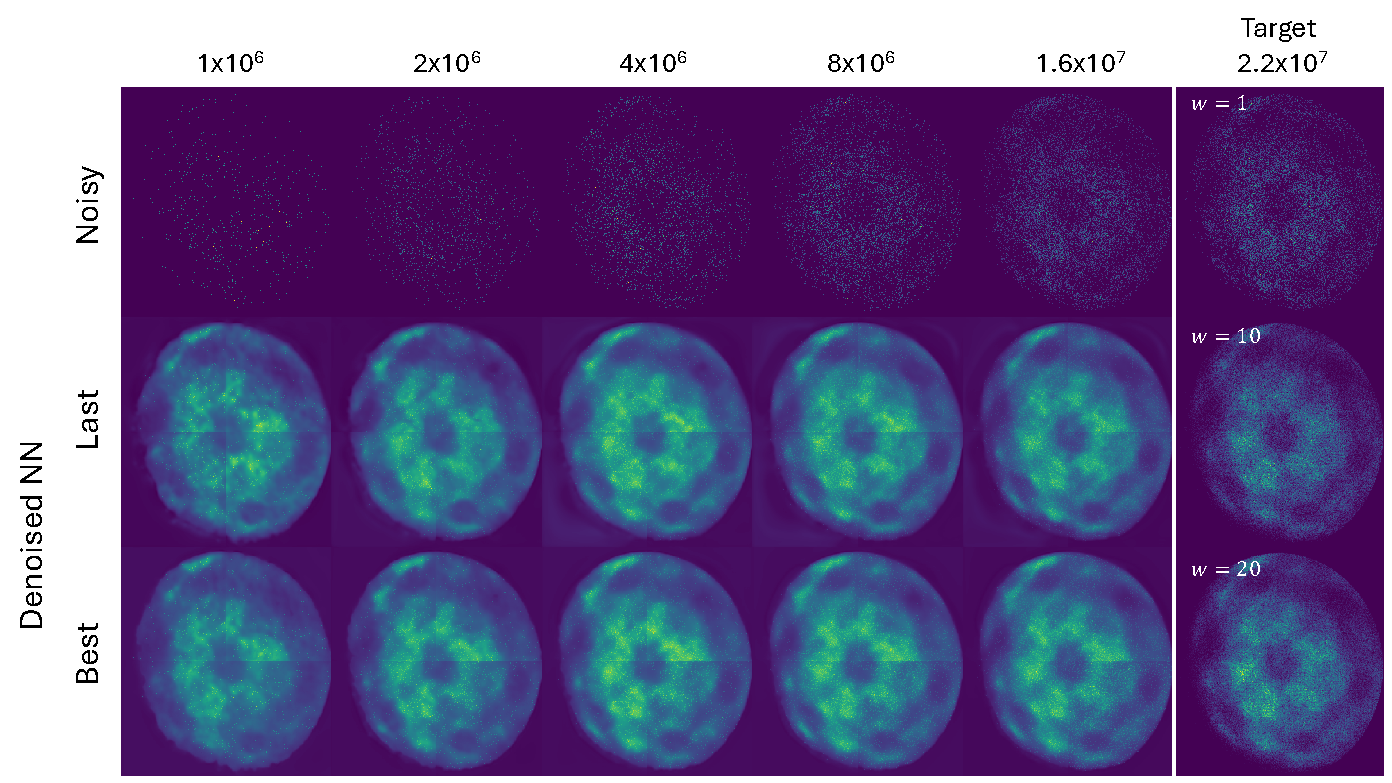
\includegraphics[width=1\linewidth]{images/nn_denoised_counts_best_last_xy.pdf}
%     \caption{}
%     \label{fig:nn-denoised-counts-best-last-xy}
% \end{figure}

% \begin{figure}[h]
%     \centering
%     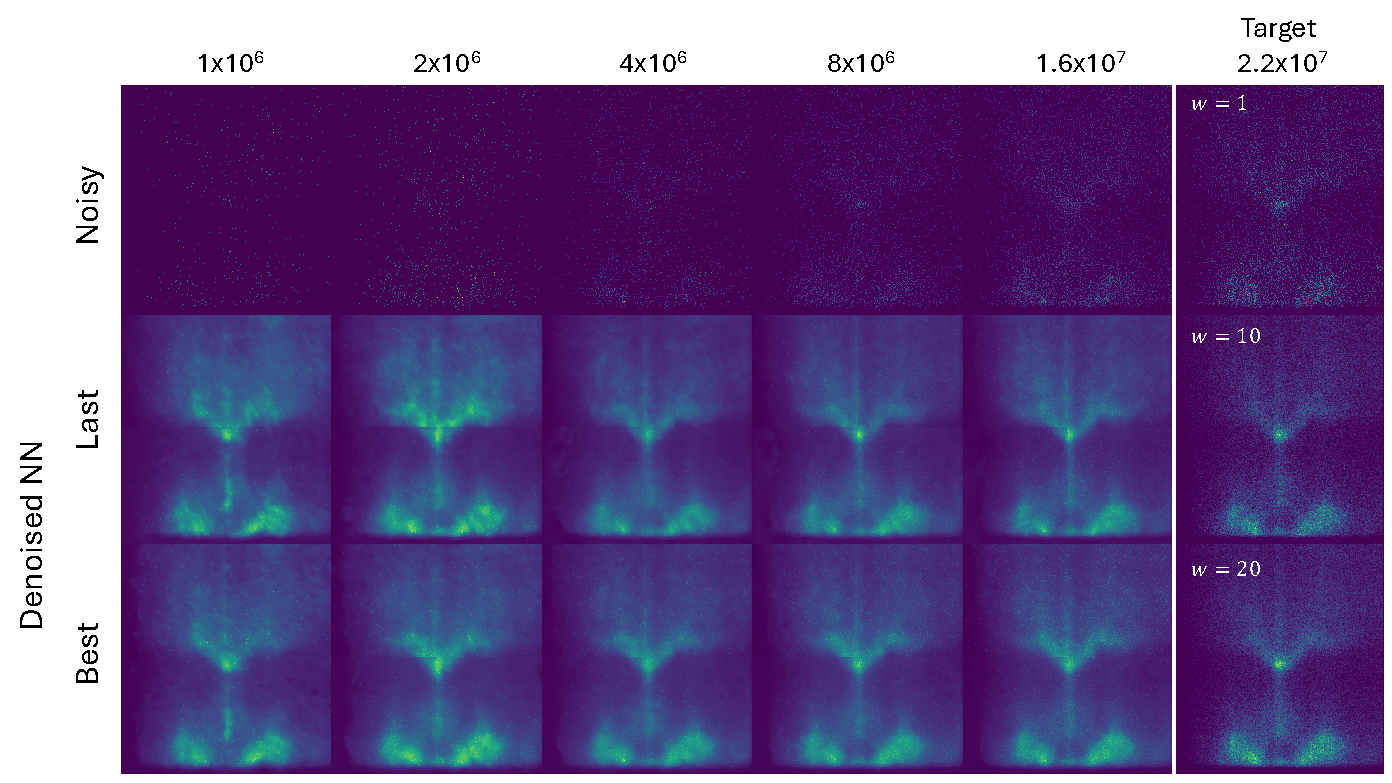
\includegraphics[width=1\linewidth]{images/nn_denoised_counts_best_last_ex.pdf}
%     \caption{}
%     \label{fig:nn-denoised-counts-best-last-ex}
% \end{figure}


